\documentclass[]{article}
\usepackage{lmodern}
\usepackage{amssymb,amsmath}
\usepackage{ifxetex,ifluatex}
\usepackage{fixltx2e} % provides \textsubscript
\ifnum 0\ifxetex 1\fi\ifluatex 1\fi=0 % if pdftex
  \usepackage[T1]{fontenc}
  \usepackage[utf8]{inputenc}
\else % if luatex or xelatex
  \ifxetex
    \usepackage{mathspec}
  \else
    \usepackage{fontspec}
  \fi
  \defaultfontfeatures{Ligatures=TeX,Scale=MatchLowercase}
\fi
% use upquote if available, for straight quotes in verbatim environments
\IfFileExists{upquote.sty}{\usepackage{upquote}}{}
% use microtype if available
\IfFileExists{microtype.sty}{%
\usepackage{microtype}
\UseMicrotypeSet[protrusion]{basicmath} % disable protrusion for tt fonts
}{}
\usepackage[margin=1in]{geometry}
\usepackage{hyperref}
\hypersetup{unicode=true,
            pdftitle={Clustering the Pharmaceutical Industry Stocks},
            pdfauthor={Hugo Toscano},
            pdfborder={0 0 0},
            breaklinks=true}
\urlstyle{same}  % don't use monospace font for urls
\usepackage{color}
\usepackage{fancyvrb}
\newcommand{\VerbBar}{|}
\newcommand{\VERB}{\Verb[commandchars=\\\{\}]}
\DefineVerbatimEnvironment{Highlighting}{Verbatim}{commandchars=\\\{\}}
% Add ',fontsize=\small' for more characters per line
\usepackage{framed}
\definecolor{shadecolor}{RGB}{248,248,248}
\newenvironment{Shaded}{\begin{snugshade}}{\end{snugshade}}
\newcommand{\KeywordTok}[1]{\textcolor[rgb]{0.13,0.29,0.53}{\textbf{#1}}}
\newcommand{\DataTypeTok}[1]{\textcolor[rgb]{0.13,0.29,0.53}{#1}}
\newcommand{\DecValTok}[1]{\textcolor[rgb]{0.00,0.00,0.81}{#1}}
\newcommand{\BaseNTok}[1]{\textcolor[rgb]{0.00,0.00,0.81}{#1}}
\newcommand{\FloatTok}[1]{\textcolor[rgb]{0.00,0.00,0.81}{#1}}
\newcommand{\ConstantTok}[1]{\textcolor[rgb]{0.00,0.00,0.00}{#1}}
\newcommand{\CharTok}[1]{\textcolor[rgb]{0.31,0.60,0.02}{#1}}
\newcommand{\SpecialCharTok}[1]{\textcolor[rgb]{0.00,0.00,0.00}{#1}}
\newcommand{\StringTok}[1]{\textcolor[rgb]{0.31,0.60,0.02}{#1}}
\newcommand{\VerbatimStringTok}[1]{\textcolor[rgb]{0.31,0.60,0.02}{#1}}
\newcommand{\SpecialStringTok}[1]{\textcolor[rgb]{0.31,0.60,0.02}{#1}}
\newcommand{\ImportTok}[1]{#1}
\newcommand{\CommentTok}[1]{\textcolor[rgb]{0.56,0.35,0.01}{\textit{#1}}}
\newcommand{\DocumentationTok}[1]{\textcolor[rgb]{0.56,0.35,0.01}{\textbf{\textit{#1}}}}
\newcommand{\AnnotationTok}[1]{\textcolor[rgb]{0.56,0.35,0.01}{\textbf{\textit{#1}}}}
\newcommand{\CommentVarTok}[1]{\textcolor[rgb]{0.56,0.35,0.01}{\textbf{\textit{#1}}}}
\newcommand{\OtherTok}[1]{\textcolor[rgb]{0.56,0.35,0.01}{#1}}
\newcommand{\FunctionTok}[1]{\textcolor[rgb]{0.00,0.00,0.00}{#1}}
\newcommand{\VariableTok}[1]{\textcolor[rgb]{0.00,0.00,0.00}{#1}}
\newcommand{\ControlFlowTok}[1]{\textcolor[rgb]{0.13,0.29,0.53}{\textbf{#1}}}
\newcommand{\OperatorTok}[1]{\textcolor[rgb]{0.81,0.36,0.00}{\textbf{#1}}}
\newcommand{\BuiltInTok}[1]{#1}
\newcommand{\ExtensionTok}[1]{#1}
\newcommand{\PreprocessorTok}[1]{\textcolor[rgb]{0.56,0.35,0.01}{\textit{#1}}}
\newcommand{\AttributeTok}[1]{\textcolor[rgb]{0.77,0.63,0.00}{#1}}
\newcommand{\RegionMarkerTok}[1]{#1}
\newcommand{\InformationTok}[1]{\textcolor[rgb]{0.56,0.35,0.01}{\textbf{\textit{#1}}}}
\newcommand{\WarningTok}[1]{\textcolor[rgb]{0.56,0.35,0.01}{\textbf{\textit{#1}}}}
\newcommand{\AlertTok}[1]{\textcolor[rgb]{0.94,0.16,0.16}{#1}}
\newcommand{\ErrorTok}[1]{\textcolor[rgb]{0.64,0.00,0.00}{\textbf{#1}}}
\newcommand{\NormalTok}[1]{#1}
\usepackage{graphicx,grffile}
\makeatletter
\def\maxwidth{\ifdim\Gin@nat@width>\linewidth\linewidth\else\Gin@nat@width\fi}
\def\maxheight{\ifdim\Gin@nat@height>\textheight\textheight\else\Gin@nat@height\fi}
\makeatother
% Scale images if necessary, so that they will not overflow the page
% margins by default, and it is still possible to overwrite the defaults
% using explicit options in \includegraphics[width, height, ...]{}
\setkeys{Gin}{width=\maxwidth,height=\maxheight,keepaspectratio}
\IfFileExists{parskip.sty}{%
\usepackage{parskip}
}{% else
\setlength{\parindent}{0pt}
\setlength{\parskip}{6pt plus 2pt minus 1pt}
}
\setlength{\emergencystretch}{3em}  % prevent overfull lines
\providecommand{\tightlist}{%
  \setlength{\itemsep}{0pt}\setlength{\parskip}{0pt}}
\setcounter{secnumdepth}{0}
% Redefines (sub)paragraphs to behave more like sections
\ifx\paragraph\undefined\else
\let\oldparagraph\paragraph
\renewcommand{\paragraph}[1]{\oldparagraph{#1}\mbox{}}
\fi
\ifx\subparagraph\undefined\else
\let\oldsubparagraph\subparagraph
\renewcommand{\subparagraph}[1]{\oldsubparagraph{#1}\mbox{}}
\fi

%%% Use protect on footnotes to avoid problems with footnotes in titles
\let\rmarkdownfootnote\footnote%
\def\footnote{\protect\rmarkdownfootnote}

%%% Change title format to be more compact
\usepackage{titling}

% Create subtitle command for use in maketitle
\newcommand{\subtitle}[1]{
  \posttitle{
    \begin{center}\large#1\end{center}
    }
}

\setlength{\droptitle}{-2em}

  \title{Clustering the Pharmaceutical Industry Stocks}
    \pretitle{\vspace{\droptitle}\centering\huge}
  \posttitle{\par}
    \author{Hugo Toscano}
    \preauthor{\centering\large\emph}
  \postauthor{\par}
      \predate{\centering\large\emph}
  \postdate{\par}
    \date{2019-03-05}


\begin{document}
\maketitle

In this post I will use two of the most popular clustering methods,
hierarchical clustering and k-means clustering, to analyse a data frame
related to the financial variables of some pharmaceutical companies.
Clustering is an unsupervised learning technique where we segment the
data and identify meaningful groups that have similar characteristics.
In our case, the goal will be to find these groups within the
pharmaceutical companies data. Like we did in the previous posts we will
start by loading the required packages to our analysis.

\emph{Note:} This data is not up-to-date and some of these companies are
no longer active.

\begin{Shaded}
\begin{Highlighting}[]
\KeywordTok{library}\NormalTok{(tidyverse) }\CommentTok{# group of packages to wrangle and visualize data}
\KeywordTok{library}\NormalTok{(cluster) }\CommentTok{# cluster analysis}
\KeywordTok{library}\NormalTok{(factoextra) }\CommentTok{# visualize clusters and principal components}
\KeywordTok{library}\NormalTok{(dendextend) }\CommentTok{# visualize dendrograms}
\KeywordTok{library}\NormalTok{(here) }\CommentTok{# create a file directory}
\KeywordTok{library}\NormalTok{(ggrepel) }\CommentTok{# repel overlapping text labels}
\KeywordTok{library}\NormalTok{(clustree) }\CommentTok{# visualize clusters}
\KeywordTok{library}\NormalTok{(FactoMineR) }\CommentTok{# explore multivariate data}
\KeywordTok{library}\NormalTok{(ggcorrplot) }\CommentTok{# visualize correlations}
\KeywordTok{library}\NormalTok{(clValid) }\CommentTok{# compute cluster metrics}
\KeywordTok{library}\NormalTok{(broom) }\CommentTok{# tidy algorithm outputs}
\KeywordTok{library}\NormalTok{(umap) }\CommentTok{# dimension reduction}
\KeywordTok{library}\NormalTok{(tidyquant) }\CommentTok{# in this case theme and color for clusters visualization}
\end{Highlighting}
\end{Shaded}

The next step is to load our file and \texttt{glimpse} it.

\begin{Shaded}
\begin{Highlighting}[]
\CommentTok{# load the file}
\NormalTok{pharmaceuticals <-}\StringTok{ }\KeywordTok{read_csv}\NormalTok{(here}\OperatorTok{::}\KeywordTok{here}\NormalTok{(}\StringTok{"pharmaceuticals.csv"}\NormalTok{))}

\CommentTok{# explore the data}
\KeywordTok{glimpse}\NormalTok{(pharmaceuticals)}
\end{Highlighting}
\end{Shaded}

\begin{verbatim}
## Observations: 21
## Variables: 14
## $ Symbol                <chr> "ABT", "AGN", "AHM", "AZN", "AVE", "BAY"...
## $ Name                  <chr> "Abbott Laboratories", "Allergan, Inc.",...
## $ Market_Cap            <dbl> 68.44, 7.58, 6.30, 67.63, 47.16, 16.90, ...
## $ Beta                  <dbl> 0.32, 0.41, 0.46, 0.52, 0.32, 1.11, 0.50...
## $ PE_Ratio              <dbl> 24.7, 82.5, 20.7, 21.5, 20.1, 27.9, 13.9...
## $ ROE                   <dbl> 26.4, 12.9, 14.9, 27.4, 21.8, 3.9, 34.8,...
## $ ROA                   <dbl> 11.8, 5.5, 7.8, 15.4, 7.5, 1.4, 15.1, 4....
## $ Asset_Turnover        <dbl> 0.7, 0.9, 0.9, 0.9, 0.6, 0.6, 0.9, 0.6, ...
## $ Leverage              <dbl> 0.42, 0.60, 0.27, 0.00, 0.34, 0.00, 0.57...
## $ Rev_Growth            <dbl> 7.54, 9.16, 7.05, 15.00, 26.81, -3.17, 2...
## $ Net_Profit_Margin     <dbl> 16.1, 5.5, 11.2, 18.0, 12.9, 2.6, 20.6, ...
## $ Median_Recommendation <chr> "Moderate Buy", "Moderate Buy", "Strong ...
## $ Location              <chr> "US", "CANADA", "UK", "UK", "FRANCE", "G...
## $ Exchange              <chr> "NYSE", "NYSE", "NYSE", "NYSE", "NYSE", ...
\end{verbatim}

We have 14 variables related to the financial information of 21
pharmaceutical companies.

\section{Data Exploration}\label{data-exploration}

Before we start with our clustering analysis, we should explore our
data. First, we will check the correlations between our numeric
variables.

\textbf{Note}: for this clustering analysis we will only use the numeric
variables.

\begin{Shaded}
\begin{Highlighting}[]
\CommentTok{# create correlation matrix}
\NormalTok{pharmaceuticals_cor <-}\StringTok{ }\NormalTok{pharmaceuticals }\OperatorTok
\StringTok{  }\KeywordTok{select_if}\NormalTok{(is.numeric) }\OperatorTok
\StringTok{  }\KeywordTok{cor}\NormalTok{()}

\CommentTok{# visualize correlations}
\KeywordTok{ggcorrplot}\NormalTok{(pharmaceuticals_cor, }
           \DataTypeTok{outline.color =} \StringTok{"grey50"}\NormalTok{, }
           \DataTypeTok{lab =} \OtherTok{TRUE}\NormalTok{,}
           \DataTypeTok{hc.order =} \OtherTok{TRUE}\NormalTok{,}
           \DataTypeTok{type =} \StringTok{"full"}\NormalTok{) }
\end{Highlighting}
\end{Shaded}

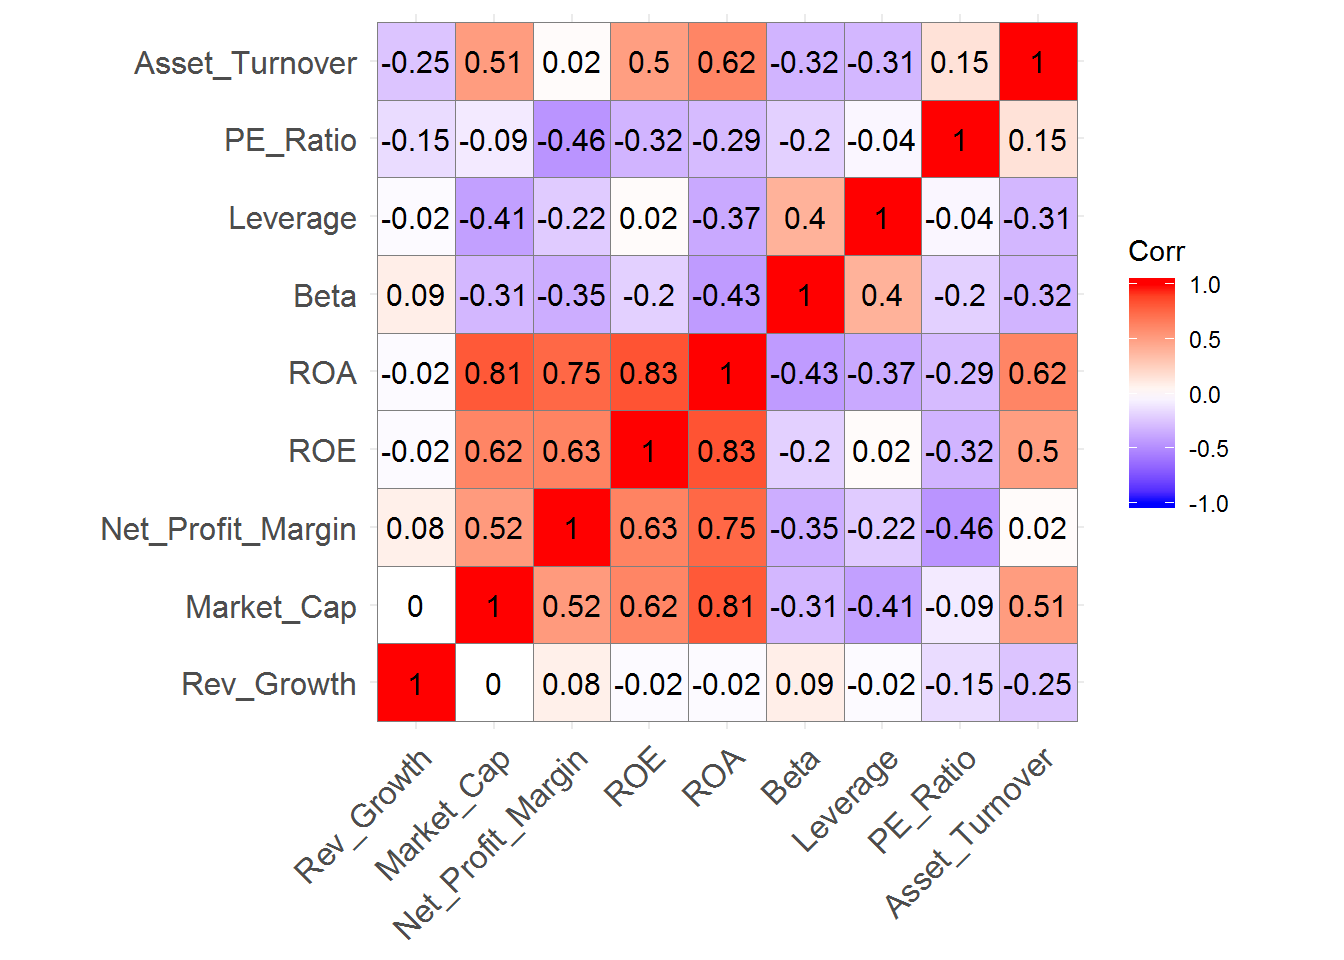
\includegraphics{2019-01-29-clustering-the-pharmaceutical-industry_files/figure-latex/unnamed-chunk-3-1.pdf}

We can identify strong positive correlations between \emph{Revenue on
Assets}, \emph{Revenue on Equity}, \emph{Net Profit Margin}, and
\emph{Market Cap} which might indicate that these variables form a
cluster.

Another way to recognize the likely number of clusters before we do our
clustering analysis is to use a Principal Component Analysis(PCA). Let's
use the \texttt{PCA} from the \texttt{FactoMineR} and the
\texttt{fviz\_screeplot} function from the \texttt{factoextra} package
to check how much variance is explained by each dimension.

\begin{Shaded}
\begin{Highlighting}[]
\CommentTok{# use a data frame only with numeric values and scale the variables because they were measured in different scales}
\NormalTok{pharmaceuticals_tbl <-}\StringTok{ }\KeywordTok{na.omit}\NormalTok{(pharmaceuticals) }\OperatorTok
\StringTok{  }\NormalTok{dplyr}\OperatorTok{::}\KeywordTok{select}\NormalTok{(}\OperatorTok{-}\KeywordTok{c}\NormalTok{(}\DecValTok{1}\NormalTok{, }\DecValTok{12}\NormalTok{, }\DecValTok{13}\NormalTok{, }\DecValTok{14}\NormalTok{)) }\OperatorTok\StringTok{ }
\StringTok{  }\KeywordTok{column_to_rownames}\NormalTok{(}\DataTypeTok{var =} \StringTok{"Name"}\NormalTok{) }\OperatorTok
\StringTok{  }\KeywordTok{scale}\NormalTok{(.) }\OperatorTok\StringTok{ }\CommentTok{# standardize the values }
\StringTok{  }\KeywordTok{as.data.frame}\NormalTok{() }\CommentTok{# convert to data frame}

\NormalTok{## use PCA to check how many dimensions we have}
\CommentTok{# PCA of our dataframe}
\NormalTok{new_pca <-}\StringTok{ }\KeywordTok{PCA}\NormalTok{(pharmaceuticals_tbl)}
\end{Highlighting}
\end{Shaded}

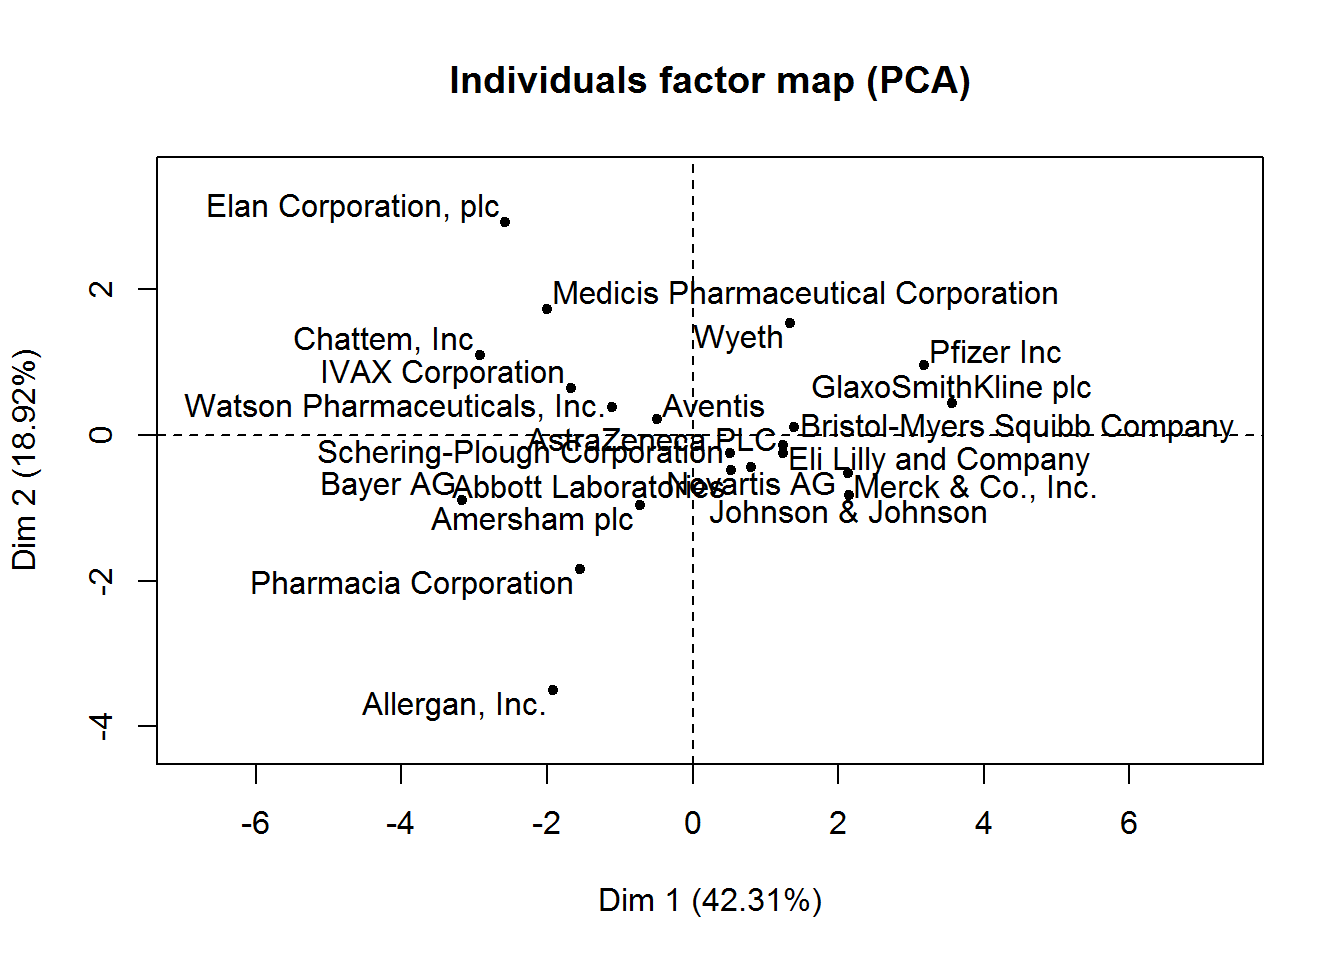
\includegraphics{2019-01-29-clustering-the-pharmaceutical-industry_files/figure-latex/unnamed-chunk-4-1.pdf}
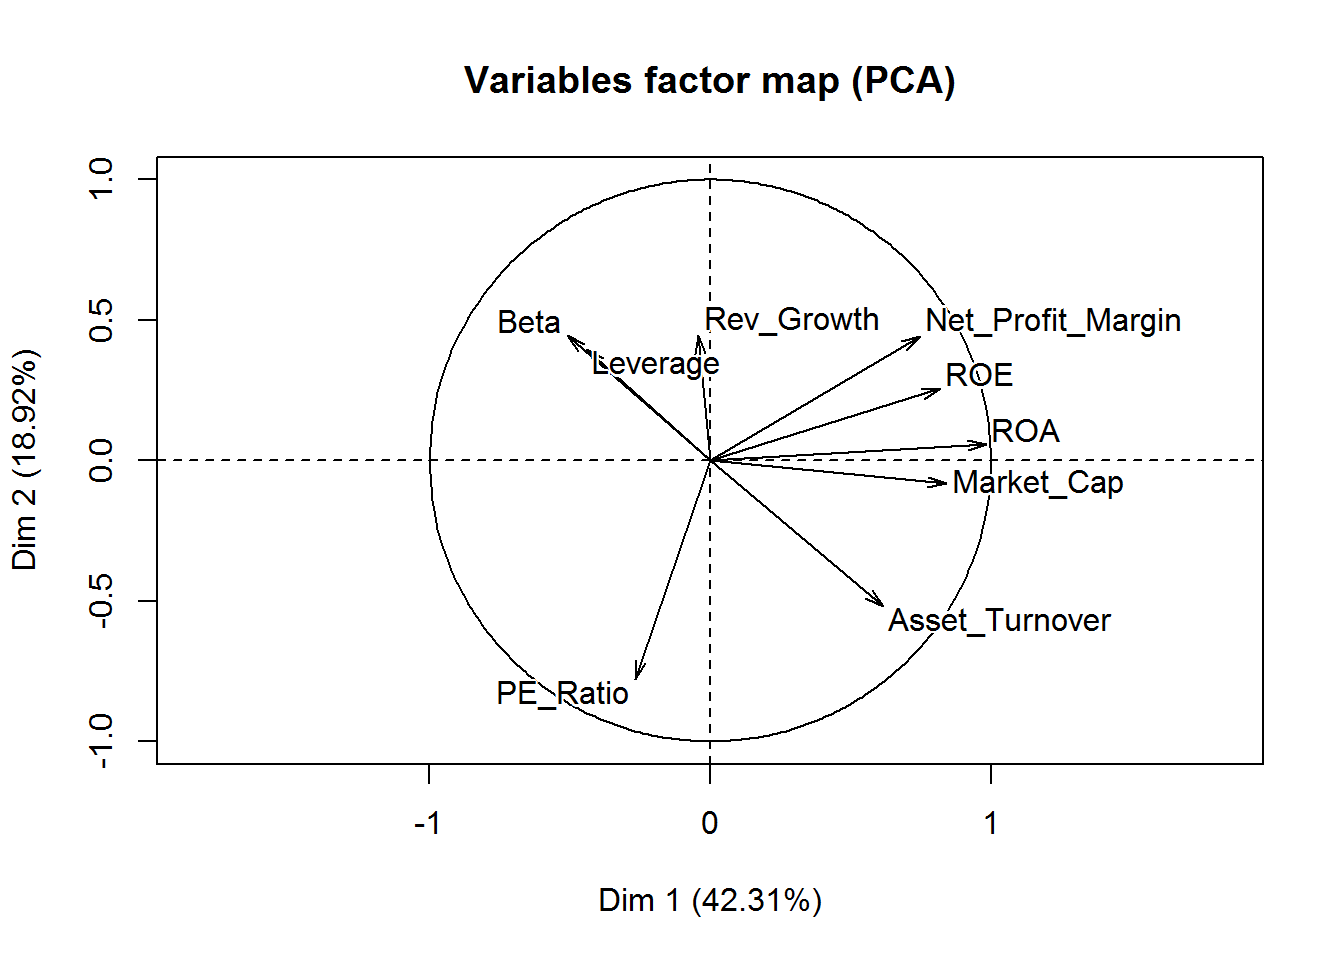
\includegraphics{2019-01-29-clustering-the-pharmaceutical-industry_files/figure-latex/unnamed-chunk-4-2.pdf}

\begin{Shaded}
\begin{Highlighting}[]
\CommentTok{# check eigenvalues and percentage of variance}
\NormalTok{new_pca}\OperatorTok{$}\NormalTok{eig}
\end{Highlighting}
\end{Shaded}

\begin{verbatim}
##        eigenvalue percentage of variance cumulative percentage of variance
## comp 1  3.8080296             42.3114401                          42.31144
## comp 2  1.7028349             18.9203881                          61.23183
## comp 3  1.1435807             12.7064523                          73.93828
## comp 4  0.8157384              9.0637604                          83.00204
## comp 5  0.7071235              7.8569272                          90.85897
## comp 6  0.4538979              5.0433098                          95.90228
## comp 7  0.2337408              2.5971197                          98.49940
## comp 8  0.1154565              1.2828502                          99.78225
## comp 9  0.0195977              0.2177522                         100.00000
\end{verbatim}

\begin{Shaded}
\begin{Highlighting}[]
\CommentTok{# visualization of how much variance each dimension explains}
\KeywordTok{fviz_screeplot}\NormalTok{(new_pca, }\DataTypeTok{addlabels =} \OtherTok{TRUE}\NormalTok{)}
\end{Highlighting}
\end{Shaded}

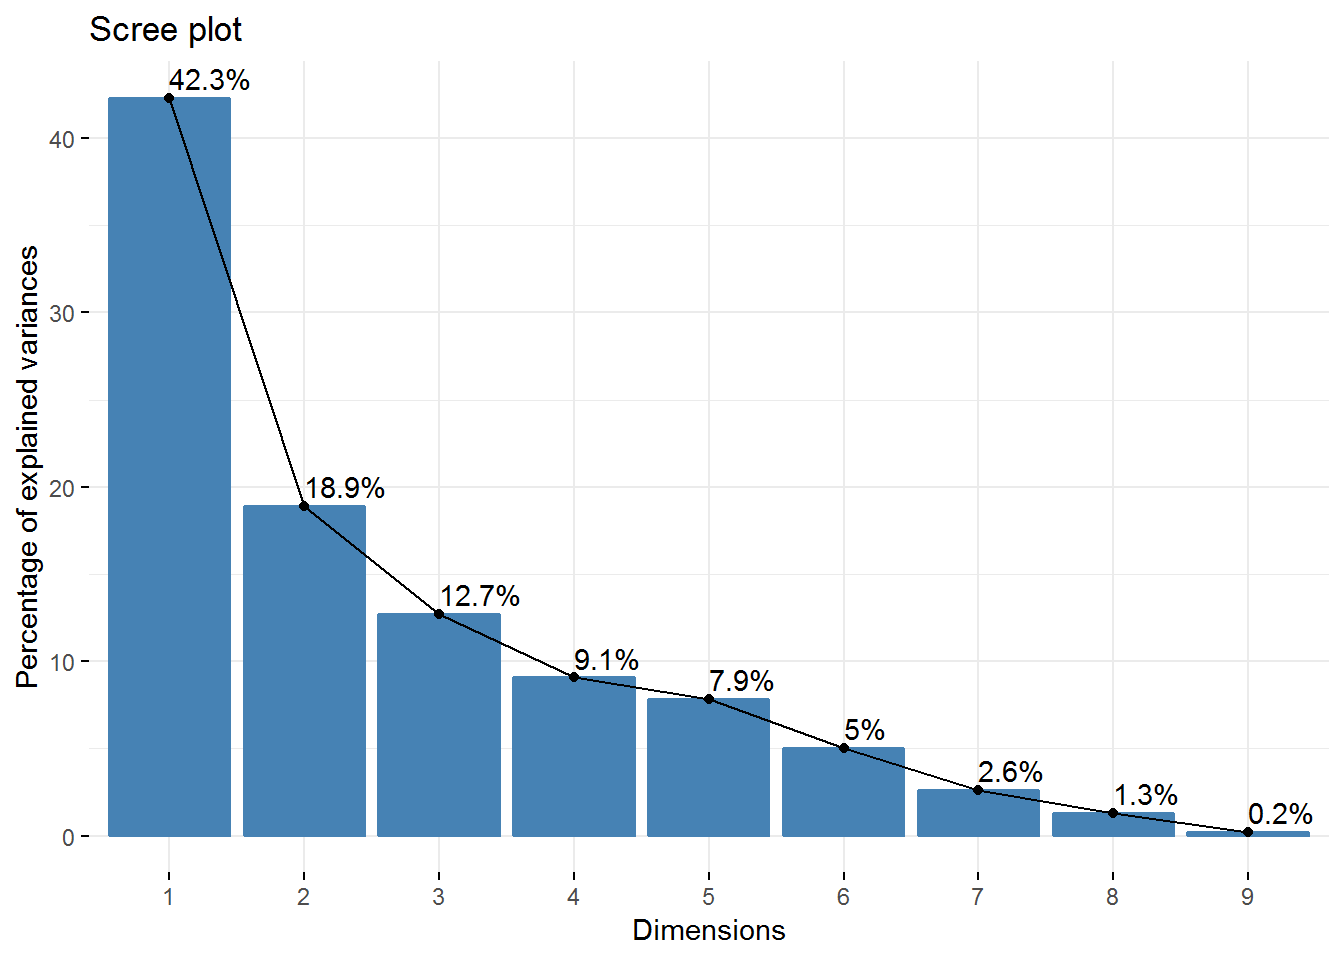
\includegraphics{2019-01-29-clustering-the-pharmaceutical-industry_files/figure-latex/unnamed-chunk-4-3.pdf}
So, we have 4 Principal Components that capture more than 80\% of the
variance. The first Principal Component explains 42.3\% and the second
18.92\%. Regarding the eigenvalues, we have 3 components with
eigenvalues above 1.

We can still check the contribution of the top 5 variables for the first
4 Principal Components using the \texttt{fviz\_contrib} function from
the \texttt{factoextra} package.

\begin{Shaded}
\begin{Highlighting}[]
\CommentTok{# get each variable PCA results}
\NormalTok{var <-}\StringTok{ }\KeywordTok{get_pca_var}\NormalTok{(new_pca)}

\CommentTok{# each variable contribution to PC1 - top 5}
\KeywordTok{fviz_contrib}\NormalTok{(new_pca, }\DataTypeTok{choice =} \StringTok{"var"}\NormalTok{, }\DataTypeTok{axes =} \DecValTok{1}\NormalTok{, }\DataTypeTok{top =} \DecValTok{5}\NormalTok{)}
\end{Highlighting}
\end{Shaded}

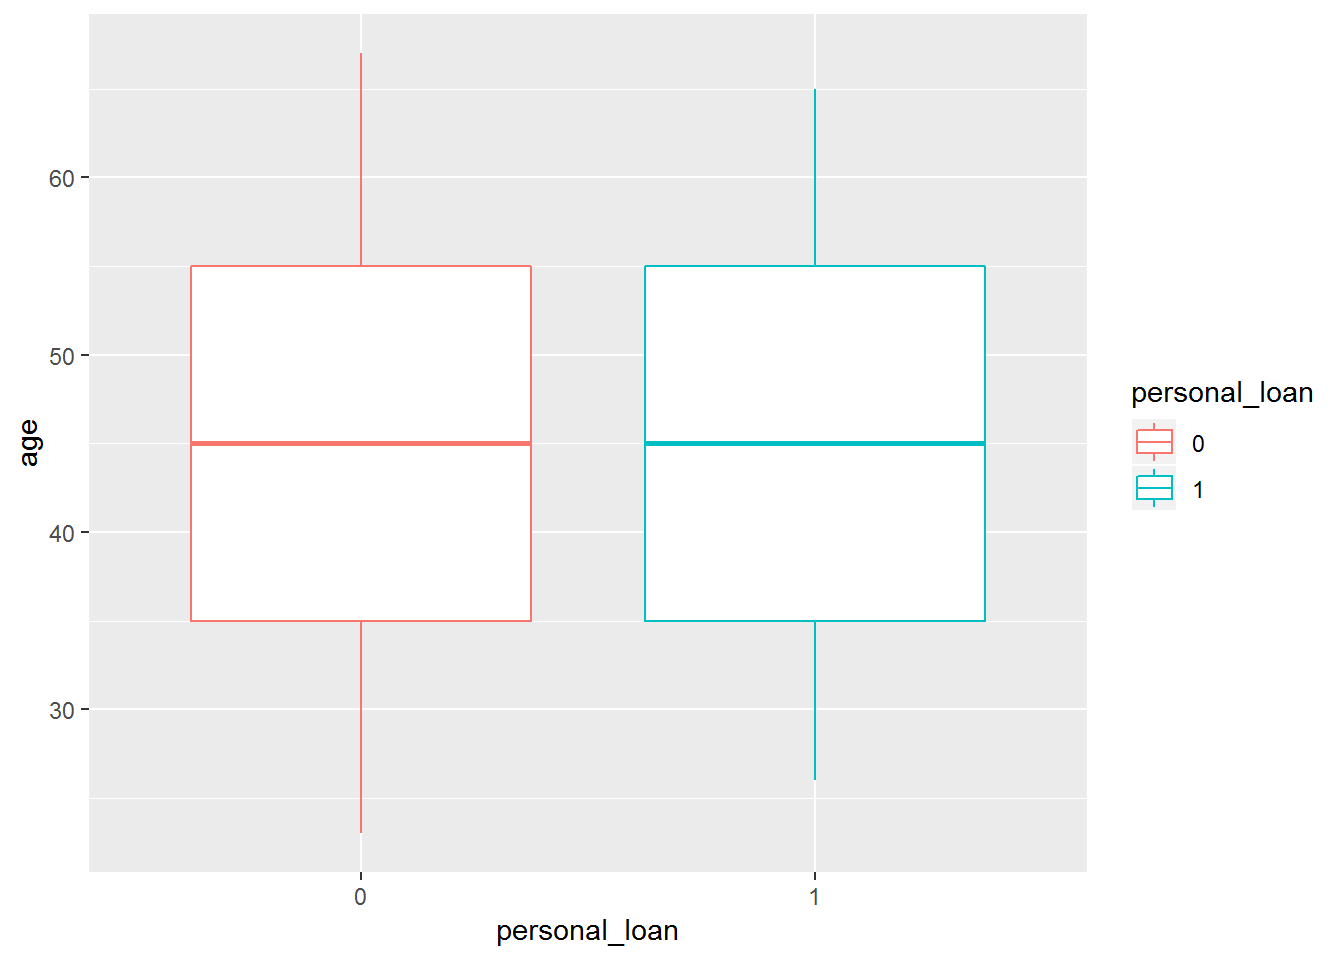
\includegraphics{2019-01-29-clustering-the-pharmaceutical-industry_files/figure-latex/unnamed-chunk-5-1.pdf}

\begin{Shaded}
\begin{Highlighting}[]
\CommentTok{# each variable contribution to PC2 - top 5}
\KeywordTok{fviz_contrib}\NormalTok{(new_pca, }\DataTypeTok{choice =} \StringTok{"var"}\NormalTok{, }\DataTypeTok{axes =} \DecValTok{2}\NormalTok{, }\DataTypeTok{top =} \DecValTok{5}\NormalTok{)}
\end{Highlighting}
\end{Shaded}

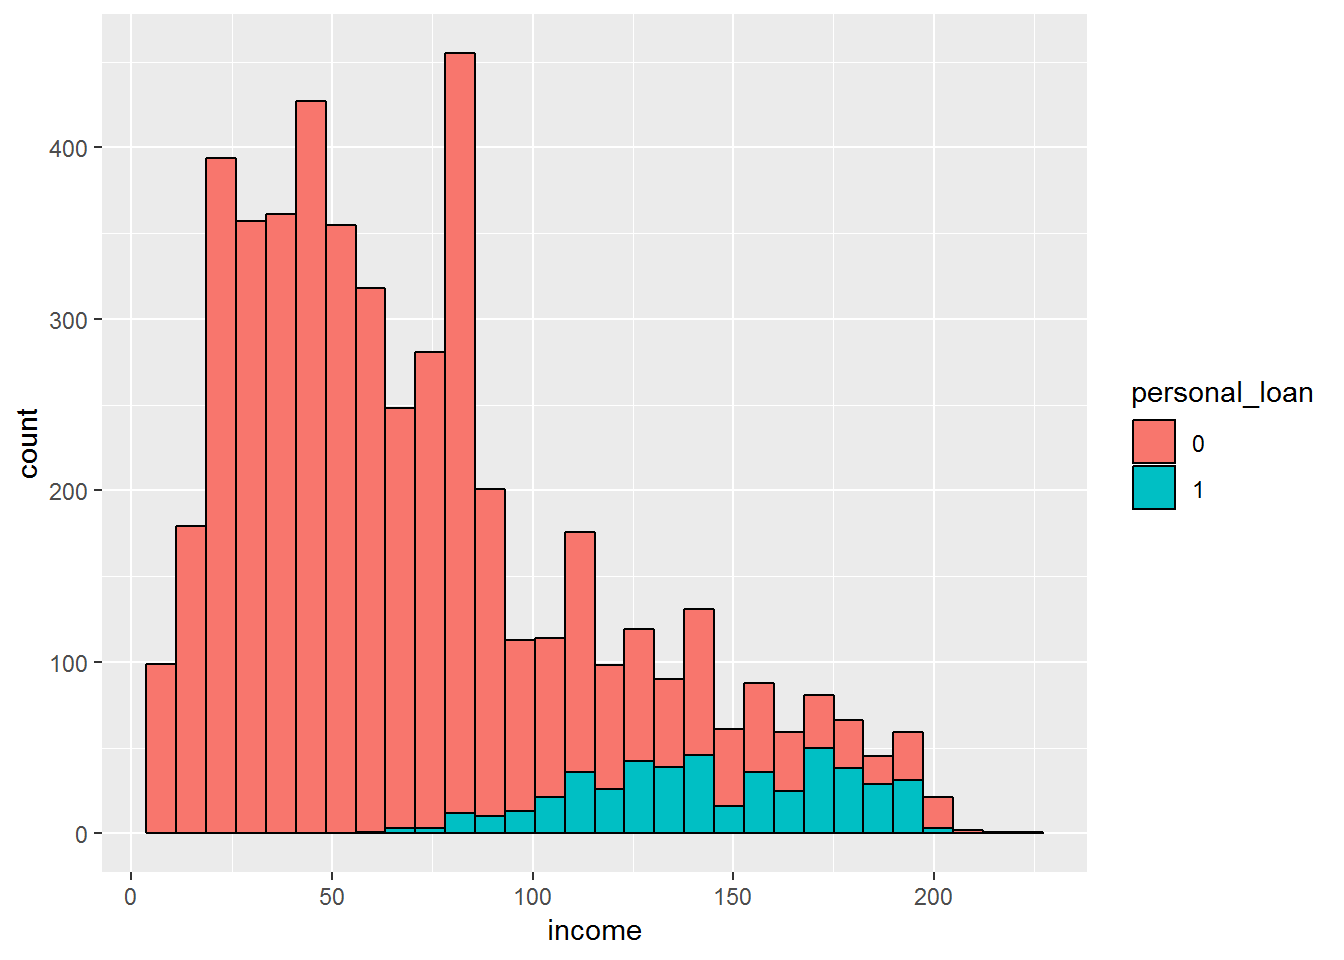
\includegraphics{2019-01-29-clustering-the-pharmaceutical-industry_files/figure-latex/unnamed-chunk-5-2.pdf}

\begin{Shaded}
\begin{Highlighting}[]
\CommentTok{# each variable contribution to PC3 - top 5}
\KeywordTok{fviz_contrib}\NormalTok{(new_pca, }\DataTypeTok{choice =} \StringTok{"var"}\NormalTok{, }\DataTypeTok{axes =} \DecValTok{3}\NormalTok{, }\DataTypeTok{top =} \DecValTok{5}\NormalTok{)}
\end{Highlighting}
\end{Shaded}

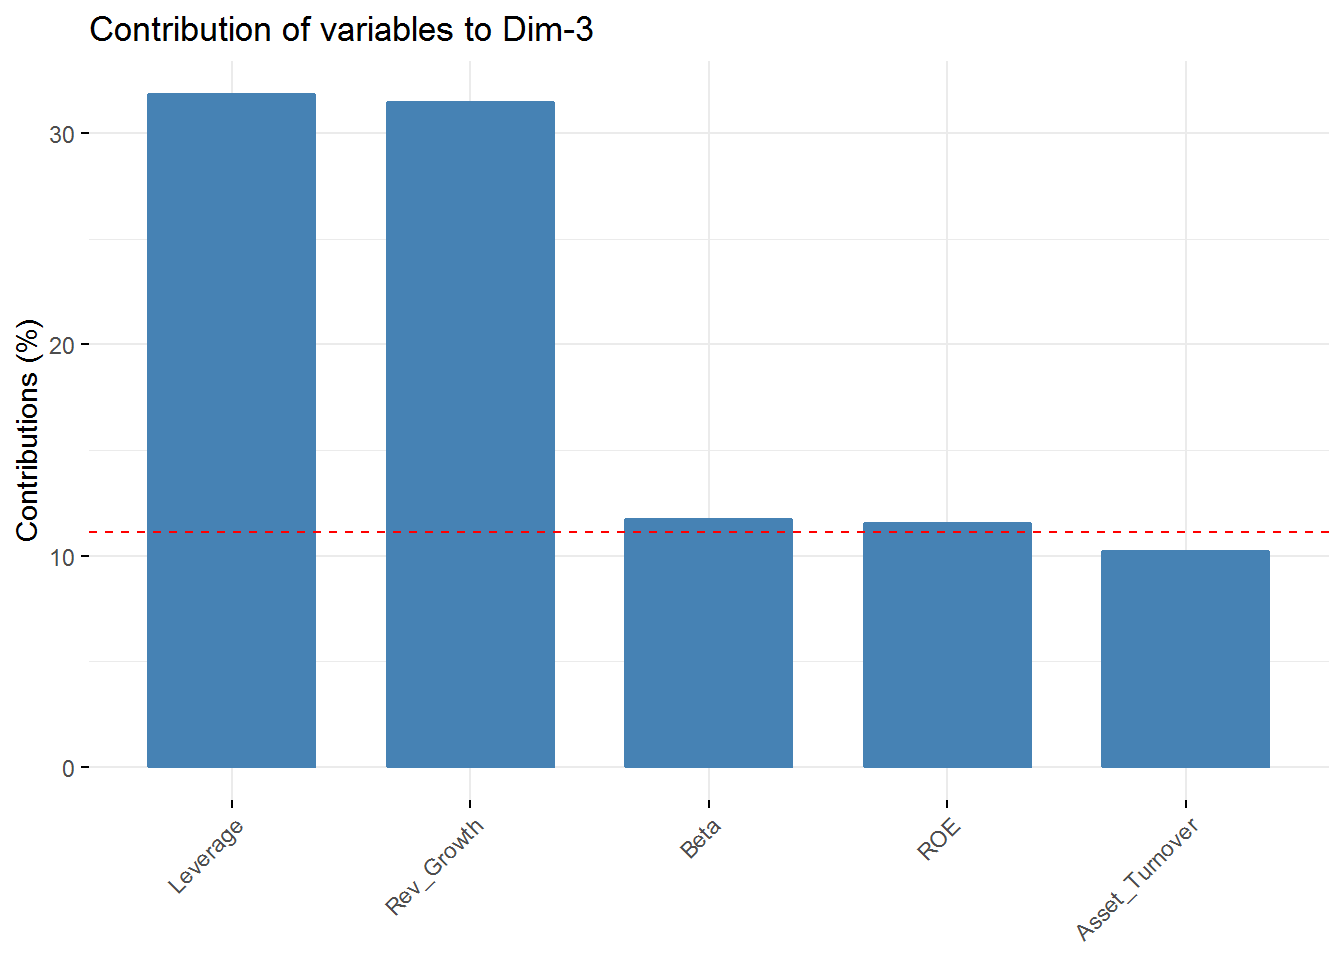
\includegraphics{2019-01-29-clustering-the-pharmaceutical-industry_files/figure-latex/unnamed-chunk-5-3.pdf}

\begin{Shaded}
\begin{Highlighting}[]
\CommentTok{# each variable contribution to PC - top 5}
\KeywordTok{fviz_contrib}\NormalTok{(new_pca, }\DataTypeTok{choice =} \StringTok{"var"}\NormalTok{, }\DataTypeTok{axes =} \DecValTok{4}\NormalTok{, }\DataTypeTok{top =} \DecValTok{5}\NormalTok{)}
\end{Highlighting}
\end{Shaded}

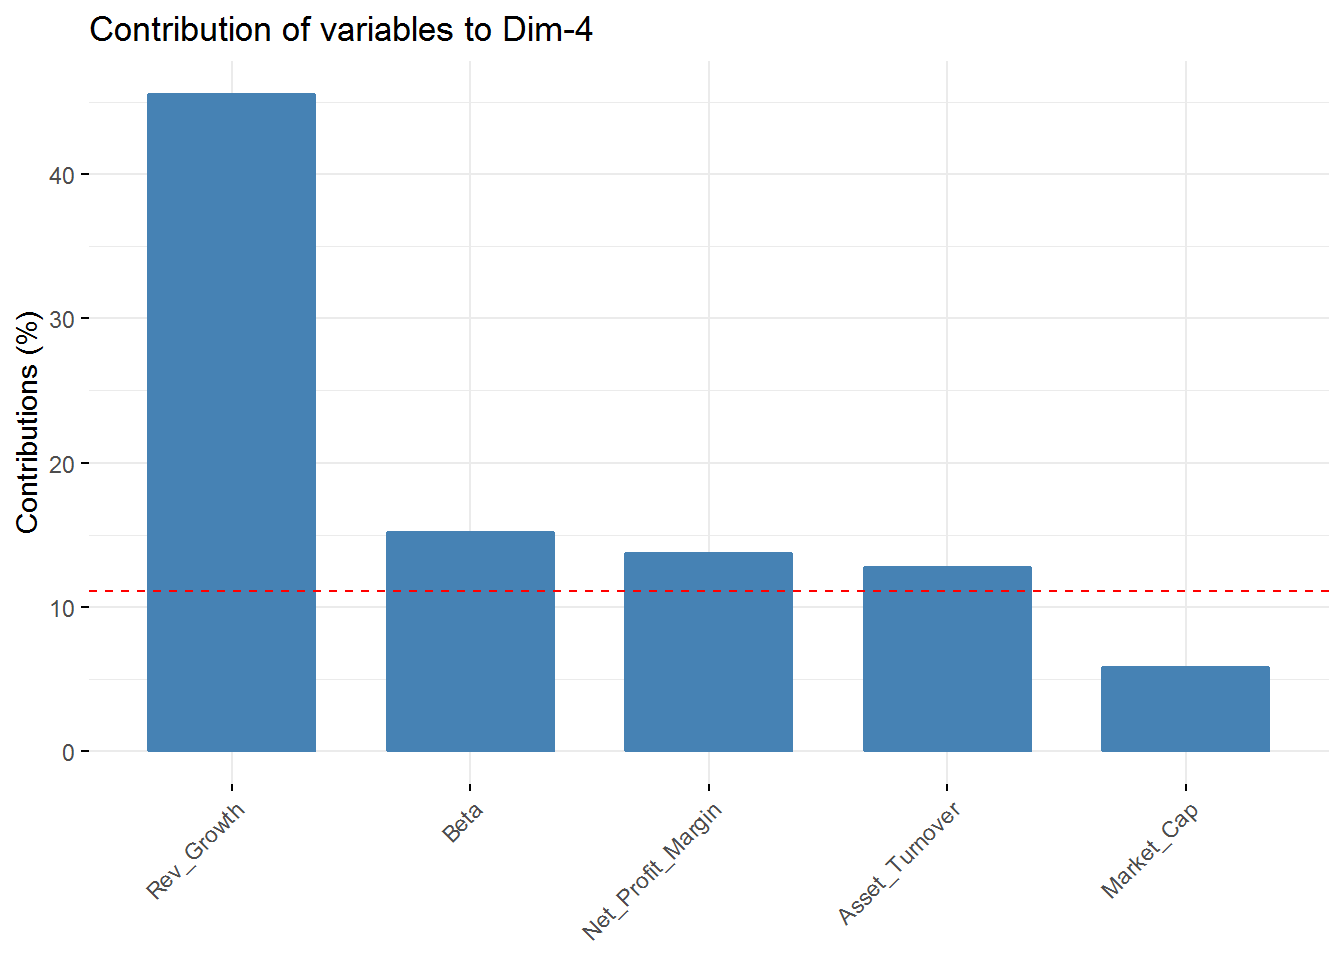
\includegraphics{2019-01-29-clustering-the-pharmaceutical-industry_files/figure-latex/unnamed-chunk-5-4.pdf}
In the first component \emph{Revenue on assets}, \emph{Market Cap},
\emph{Revenue on Equity}, and \emph{Net Profit Margin} are the variables
with highest contribution. For the second component,
\emph{Price/Earnings Ratio} and \emph{Asset turnover} are the highest
contributors. In the third component \emph{Leverage} and \emph{Revenue
Growth} have the highest contribution. Finally, in the fourth component
the variables with the highest contribution are \emph{Revenue Growth}
and \emph{Beta}.

Visualize the contribution of the variables for the first two components
is possible through an axis.

\begin{Shaded}
\begin{Highlighting}[]
\CommentTok{# visualization of the first two components and the contributions of each variable}
\KeywordTok{fviz_pca_var}\NormalTok{(new_pca, }\DataTypeTok{col.var=}\StringTok{"contrib"}\NormalTok{,}
             \DataTypeTok{gradient.cols =} \KeywordTok{c}\NormalTok{(}\StringTok{"red"}\NormalTok{, }\StringTok{"green"}\NormalTok{, }\StringTok{"blue"}\NormalTok{),}
             \DataTypeTok{repel =} \OtherTok{TRUE} 
\NormalTok{             ) }\OperatorTok{+}\StringTok{ }
\StringTok{  }\KeywordTok{labs}\NormalTok{( }\DataTypeTok{title =} \StringTok{"Variables - PCA"}\NormalTok{)}
\end{Highlighting}
\end{Shaded}

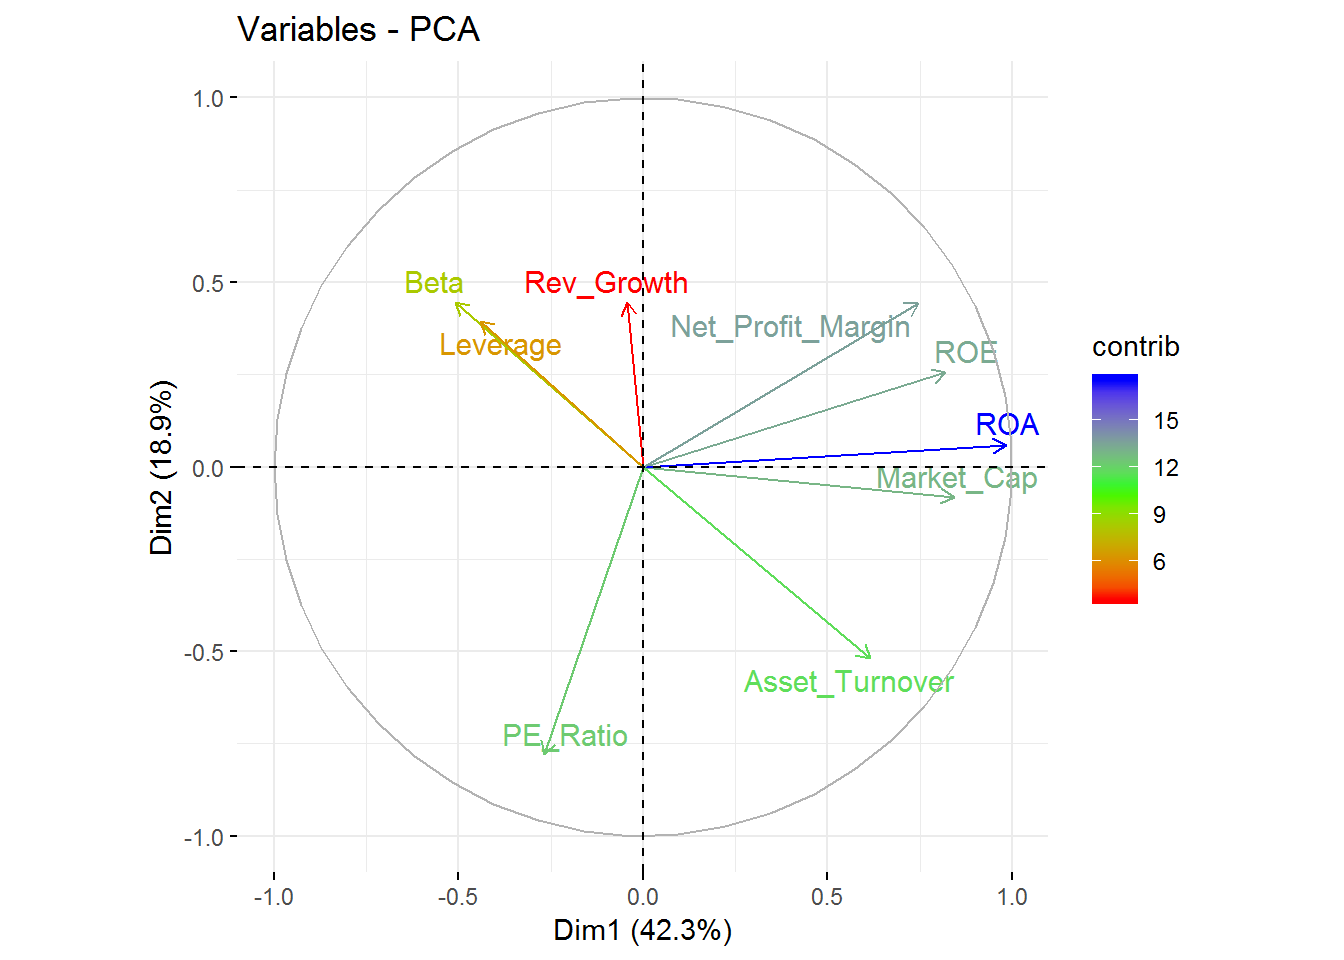
\includegraphics{2019-01-29-clustering-the-pharmaceutical-industry_files/figure-latex/unnamed-chunk-6-1.pdf}

From this visualization, it's clear that \emph{Revenue on assets},
\emph{Revenue on equity}, \emph{Net Profit Margin}, \emph{Market Cap},
and \emph{Asset Turnover} tend to increase together and are the highest
contributors to the first component.

Following the exploration of our data, let's us start our clustering
analysis.

\subsection{Hierarchical Cluster
Analysis}\label{hierarchical-cluster-analysis}

Hierarchical clustering is an approach to identify groups within a data
frame where there is noneed to pre-specify the number of clusters
intended to be extracted.

As we have already scaled our data including the removal of any missing
values, we can start our clustering process. First, we should measure
the similarity between our observations using an \emph{euclidean}
distance measure - other measures can be used such as the Manhattan
distance. These distances can be visualized with the function
\texttt{fviz\_dist} from the \texttt{factoextra}.

\begin{Shaded}
\begin{Highlighting}[]
\CommentTok{# compute distance measure}
\NormalTok{dt <-}\StringTok{ }\KeywordTok{dist}\NormalTok{(pharmaceuticals_tbl, }\DataTypeTok{method =} \StringTok{"euclidean"}\NormalTok{)}


\CommentTok{# visualize distance}
\KeywordTok{fviz_dist}\NormalTok{(dt, }\DataTypeTok{gradient =} \KeywordTok{list}\NormalTok{(}\DataTypeTok{low =} \StringTok{"red"}\NormalTok{, }\DataTypeTok{mid =} \StringTok{"white"}\NormalTok{, }\DataTypeTok{high =} \StringTok{"blue"}\NormalTok{))}
\end{Highlighting}
\end{Shaded}

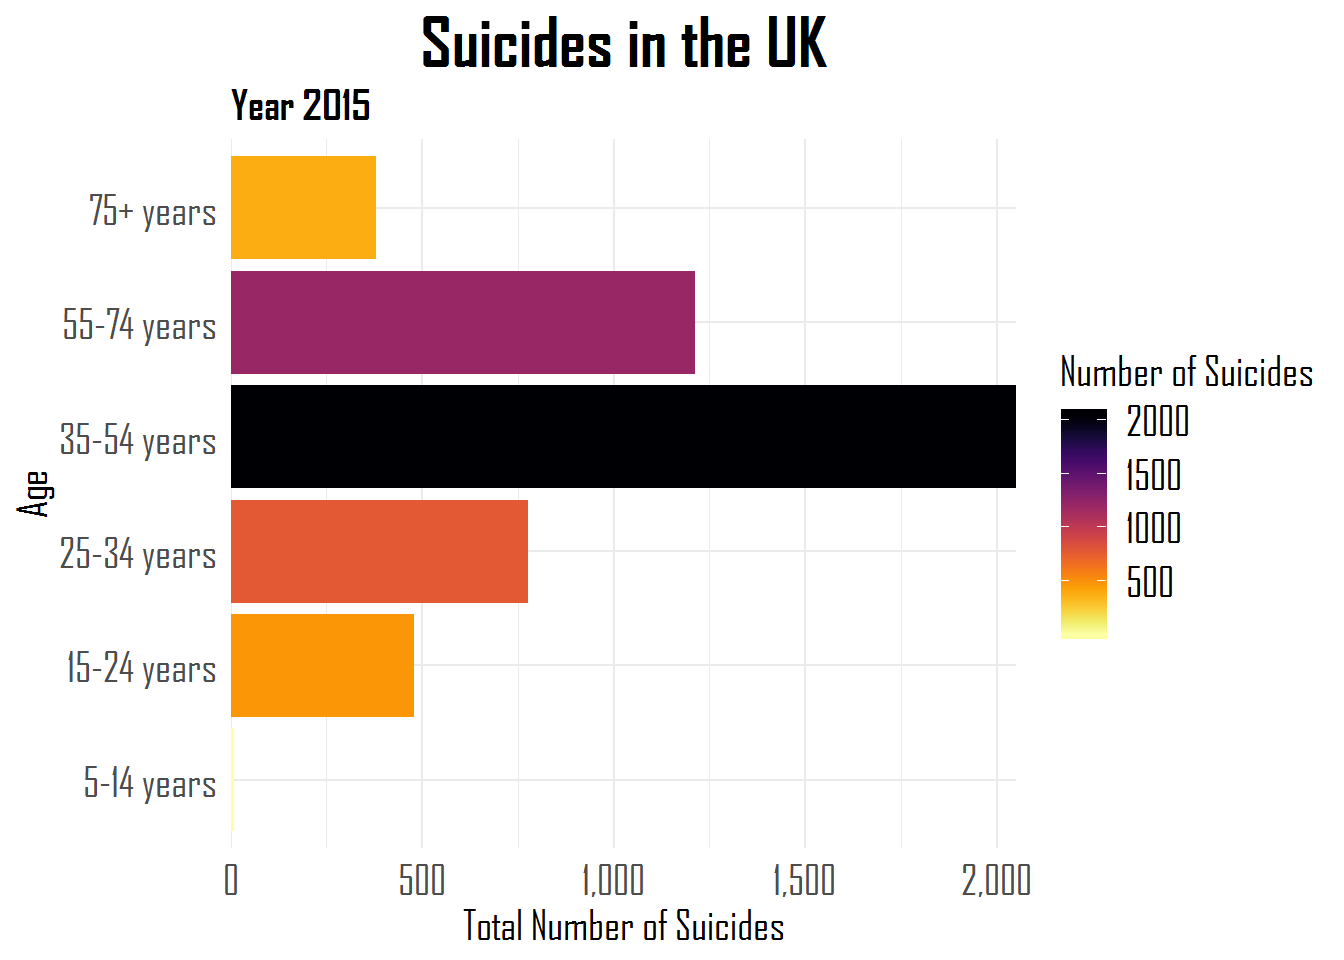
\includegraphics{2019-01-29-clustering-the-pharmaceutical-industry_files/figure-latex/unnamed-chunk-7-1.pdf}

Choosing a method of linkage is the next step. It can be:
\emph{complete} which considers the maximal distance between clusters,
\emph{simple} where is taken into account the smallest distance between
clusters, \emph{average} where the average distance between clusters is
considered, and \emph{ward} method where the pair of clusters with the
lowest distance is merged. We can create a function with \texttt{agnes}
function - it's also an agglomerative hierarchical clustering method -
to check which method gives higher agglomerative coefficient, that is, a
greater clustering structure.

\begin{Shaded}
\begin{Highlighting}[]
\NormalTok{m <-}\StringTok{ }\KeywordTok{c}\NormalTok{(}\StringTok{"average"}\NormalTok{, }\StringTok{"single"}\NormalTok{, }\StringTok{"complete"}\NormalTok{, }\StringTok{"ward"}\NormalTok{)}
\KeywordTok{names}\NormalTok{(m) <-}\StringTok{ }\KeywordTok{c}\NormalTok{(}\StringTok{"average"}\NormalTok{, }\StringTok{"single"}\NormalTok{, }\StringTok{"complete"}\NormalTok{, }\StringTok{"ward"}\NormalTok{)}


\CommentTok{#function to check the best (means higher value) linkage method }
\NormalTok{ac <-}\StringTok{ }\ControlFlowTok{function}\NormalTok{(x) \{}
  \KeywordTok{agnes}\NormalTok{(dt, }\DataTypeTok{method =}\NormalTok{ x)}\OperatorTok{$}\NormalTok{ac}
\NormalTok{\}}

\KeywordTok{map_dbl}\NormalTok{(m, ac)}
\end{Highlighting}
\end{Shaded}

\begin{verbatim}
##   average    single  complete      ward 
## 0.5600652 0.4600348 0.6990833 0.7943164
\end{verbatim}

Thus, the \emph{ward} method give us a higher agglomerative coefficient.
From now on, we will use this linkage method in our hierarchical
clustering analysis.

\begin{Shaded}
\begin{Highlighting}[]
\CommentTok{# hierarchical clustering }
\KeywordTok{set.seed}\NormalTok{(}\DecValTok{88}\NormalTok{)}
\NormalTok{hclust_}\DecValTok{1}\NormalTok{ <-}\StringTok{ }\KeywordTok{hclust}\NormalTok{(dt, }\DataTypeTok{method =} \StringTok{"ward.D2"}\NormalTok{) }\CommentTok{# ward.D2 corresponds to the ward                                                method in the hclust function}

\CommentTok{# plot hierarchical clustering}
\KeywordTok{plot}\NormalTok{(hclust_}\DecValTok{1}\NormalTok{, }\DataTypeTok{cex =} \FloatTok{0.6}\NormalTok{)}
\end{Highlighting}
\end{Shaded}

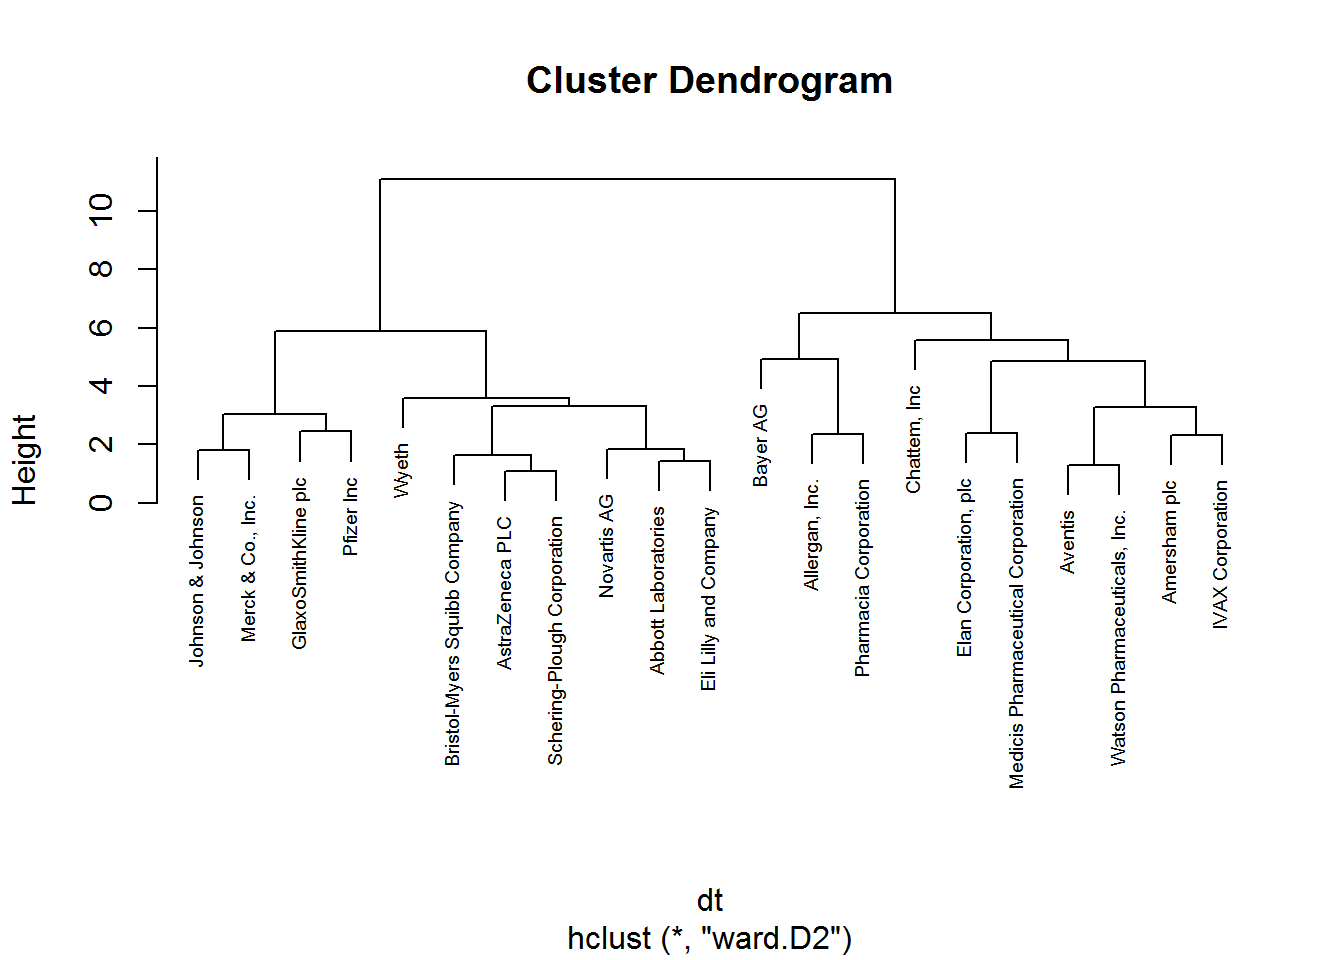
\includegraphics{2019-01-29-clustering-the-pharmaceutical-industry_files/figure-latex/unnamed-chunk-9-1.pdf}

Now, we should determine the optimal number of clusters - this process
will also be used to determine the number of clusters in the following
k-means algorithm. We will use two methods: \emph{elbow} and
\emph{average silhouette}.

\begin{Shaded}
\begin{Highlighting}[]
\CommentTok{# elbow method}
\KeywordTok{fviz_nbclust}\NormalTok{(pharmaceuticals_tbl, }\DataTypeTok{FUNcluster =}\NormalTok{ hcut, }\DataTypeTok{method =} \StringTok{"wss"}\NormalTok{)}
\end{Highlighting}
\end{Shaded}

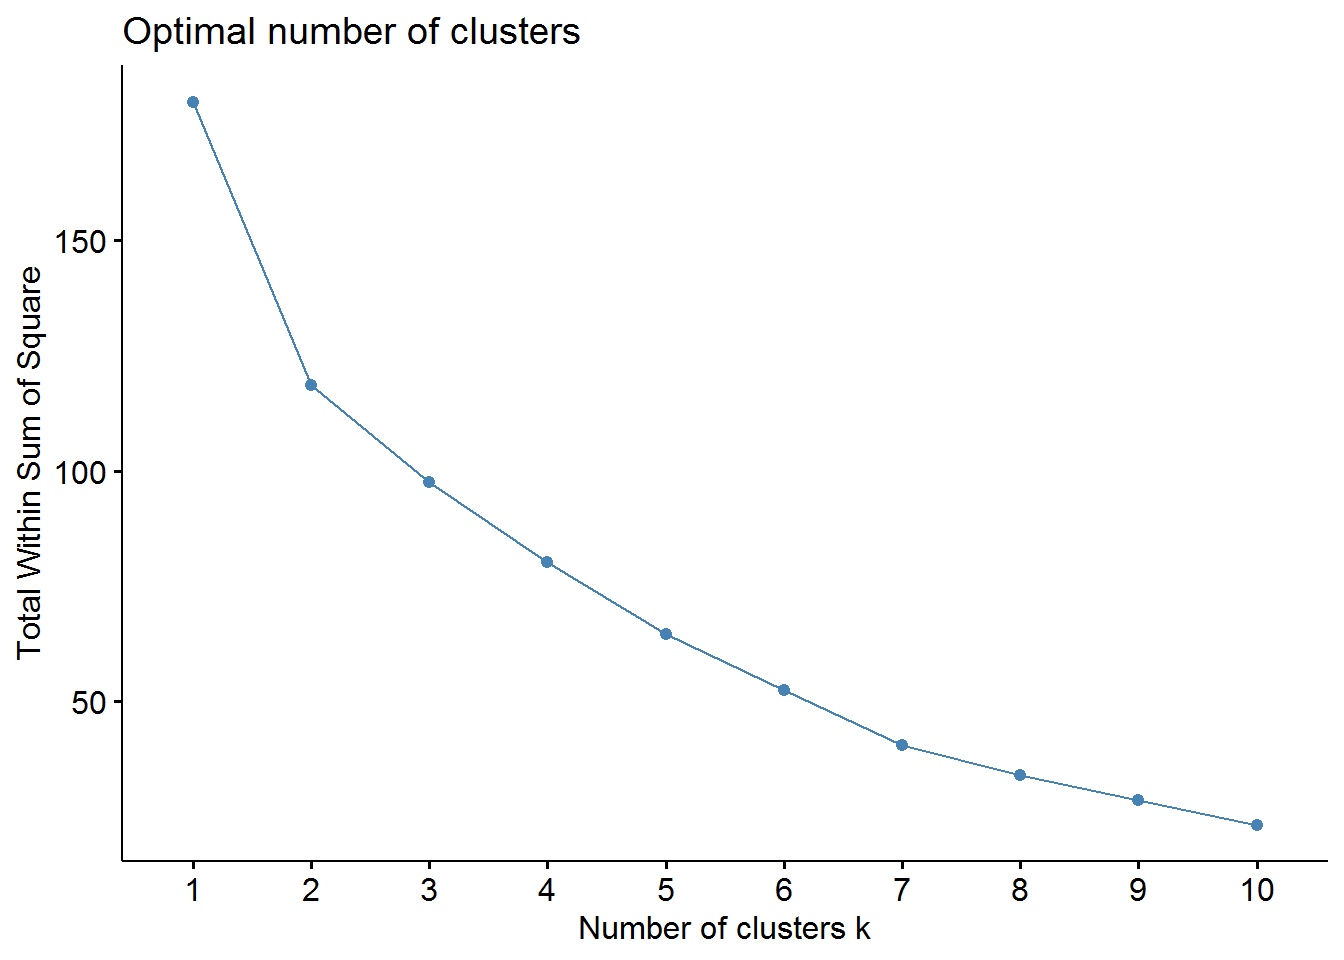
\includegraphics{2019-01-29-clustering-the-pharmaceutical-industry_files/figure-latex/unnamed-chunk-10-1.pdf}

\begin{Shaded}
\begin{Highlighting}[]
\CommentTok{# sillhouette method}
\KeywordTok{fviz_nbclust}\NormalTok{(pharmaceuticals_tbl, }\DataTypeTok{FUNcluster =}\NormalTok{ hcut, }\DataTypeTok{method =} \StringTok{"silhouette"}\NormalTok{)}
\end{Highlighting}
\end{Shaded}

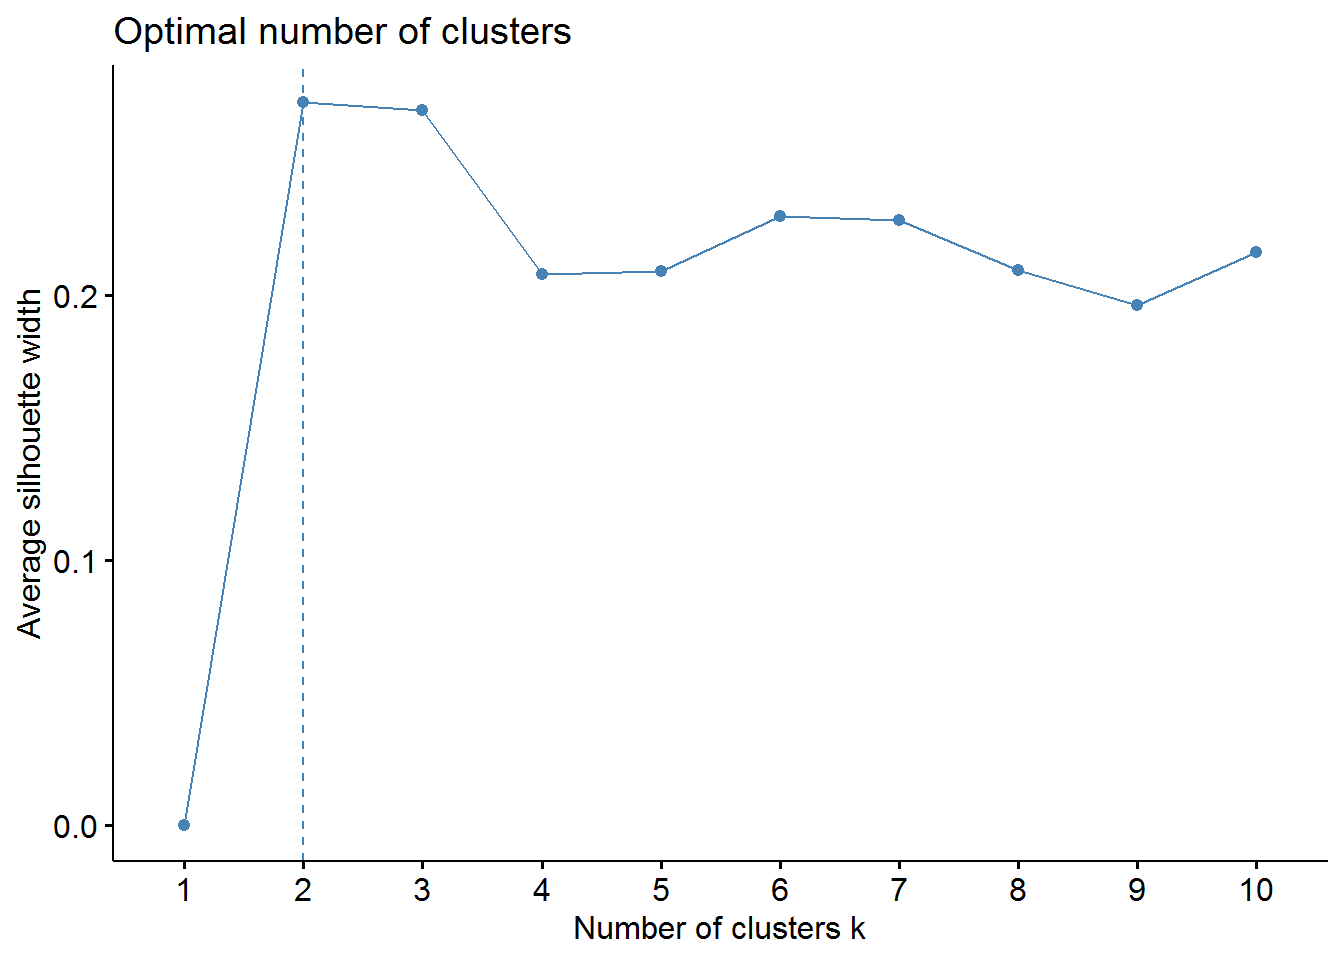
\includegraphics{2019-01-29-clustering-the-pharmaceutical-industry_files/figure-latex/unnamed-chunk-10-2.pdf}

From these visualizations we should have two clusters. Let's use the
\texttt{cutree} function to cut our dendogram in 2 clusters.

\begin{Shaded}
\begin{Highlighting}[]
\CommentTok{# cutree function}
\NormalTok{cl_}\DecValTok{1}\NormalTok{ <-}\StringTok{ }\KeywordTok{cutree}\NormalTok{(hclust_}\DecValTok{1}\NormalTok{, }\DataTypeTok{k =} \DecValTok{2}\NormalTok{)}

\CommentTok{# table function check the number of pharmaceutical companies in each cluster}
\KeywordTok{table}\NormalTok{(cl_}\DecValTok{1}\NormalTok{)}
\end{Highlighting}
\end{Shaded}

\begin{verbatim}
## cl_1
##  1  2 
## 11 10
\end{verbatim}

Consequently, 11 and 10 companies are displayed in \emph{cluster 1} and
\emph{cluster 2} respectively.

More important, we can visualize how the pharmaceutical companies are
distributed in each cluster.

\begin{Shaded}
\begin{Highlighting}[]
\KeywordTok{plot}\NormalTok{(hclust_}\DecValTok{1}\NormalTok{, }\DataTypeTok{cex =} \FloatTok{0.6}\NormalTok{)}
\KeywordTok{rect.hclust}\NormalTok{(hclust_}\DecValTok{1}\NormalTok{, }\DataTypeTok{k =} \DecValTok{2}\NormalTok{, }\DataTypeTok{border=} \DecValTok{2}\OperatorTok{:}\DecValTok{5}\NormalTok{)}
\end{Highlighting}
\end{Shaded}

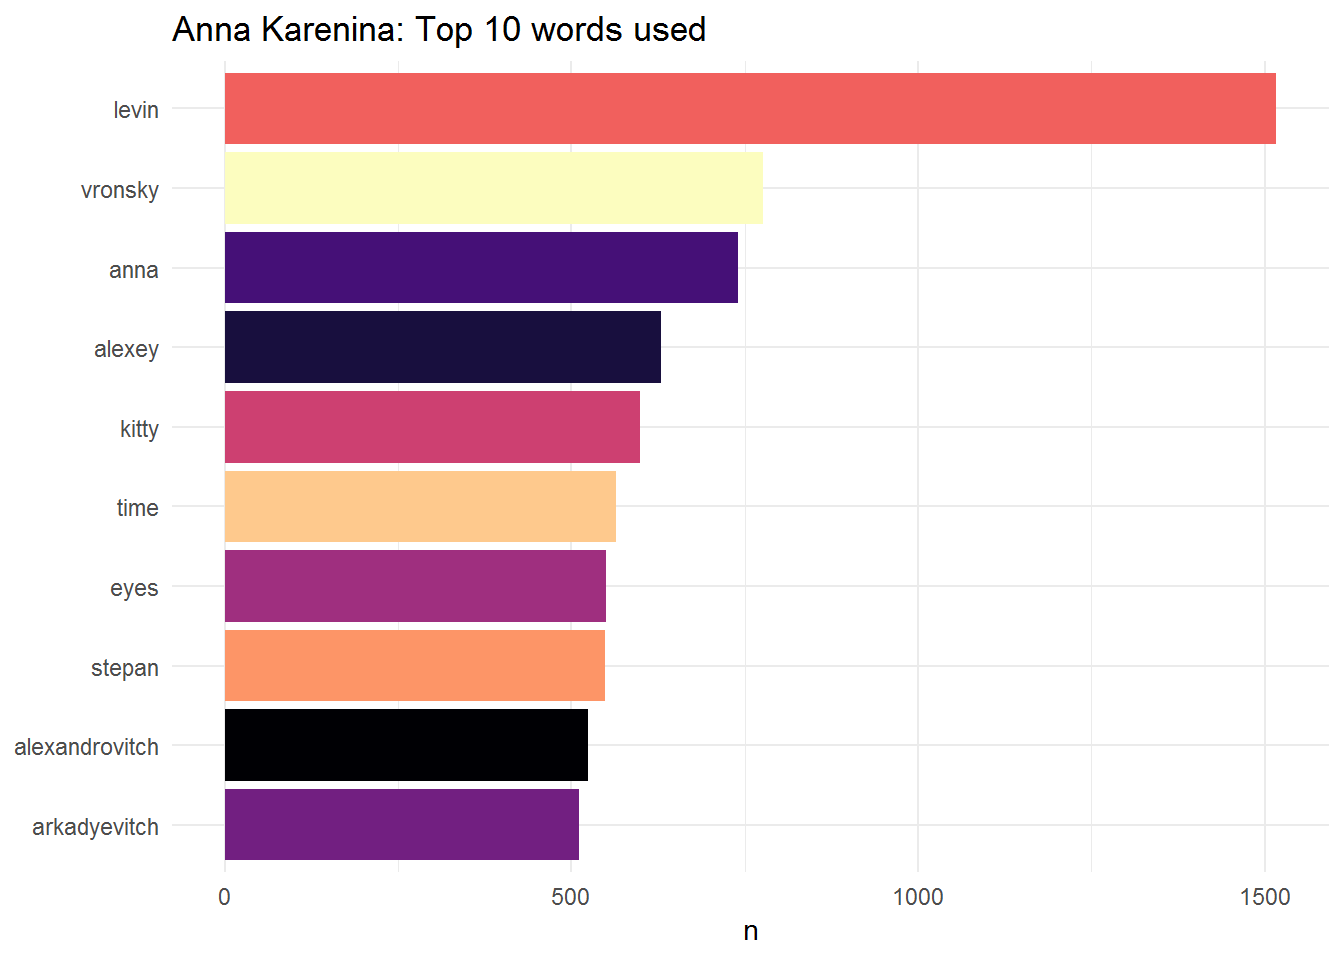
\includegraphics{2019-01-29-clustering-the-pharmaceutical-industry_files/figure-latex/unnamed-chunk-12-1.pdf}

We can also visualize in a two-dimensional graph our two clusters.

\begin{Shaded}
\begin{Highlighting}[]
\CommentTok{# fviz_cluster function to visualize the clusters}
\KeywordTok{fviz_cluster}\NormalTok{(}\KeywordTok{list}\NormalTok{(}\DataTypeTok{data =}\NormalTok{ pharmaceuticals_tbl, }\DataTypeTok{cluster =}\NormalTok{ cl_}\DecValTok{1}\NormalTok{, }\DataTypeTok{repel =} \OtherTok{TRUE}\NormalTok{)) }\OperatorTok{+}
\StringTok{  }\KeywordTok{theme_minimal}\NormalTok{()}
\end{Highlighting}
\end{Shaded}

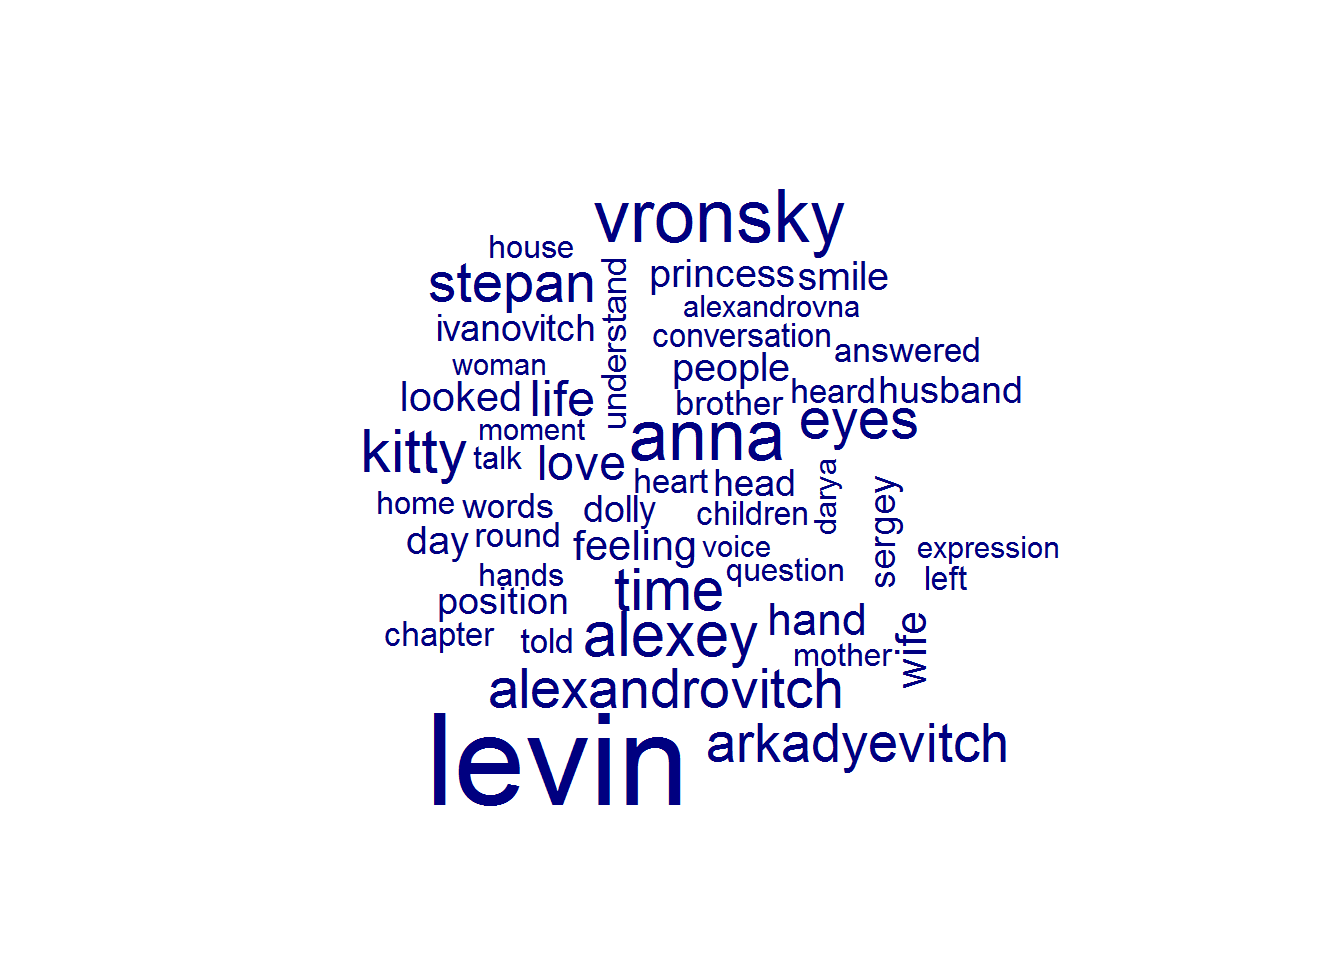
\includegraphics{2019-01-29-clustering-the-pharmaceutical-industry_files/figure-latex/unnamed-chunk-13-1.pdf}

Now that we have our clusters and recognize the pharmaceutical companies
belonging to each one, we need to check the most relevant
characteristics and describe each cluster better. However, we still need
to understand what each cluster is really about. For this, we need to
create a cluster variable in our cutree cluster dataframe generated
before. Afterwards, we should aggregate our data by cluster and verify
the mean of each variable.

\begin{Shaded}
\begin{Highlighting}[]
\CommentTok{# create cluster variable}
\NormalTok{pharmaceuticals_tbl}\OperatorTok{$}\NormalTok{cluster <-}\StringTok{ }\NormalTok{cl_}\DecValTok{1}

\CommentTok{# aggregate by cluster our variables}
\NormalTok{pharmaceuticals_tbl }\OperatorTok
\StringTok{  }\KeywordTok{group_by}\NormalTok{(cluster) }\OperatorTok
\StringTok{  }\KeywordTok{summarise_all}\NormalTok{(mean)}
\end{Highlighting}
\end{Shaded}

\begin{verbatim}
## # A tibble: 2 x 10
##   cluster Market_Cap   Beta PE_Ratio    ROE    ROA Asset_Turnover Leverage
##     <int>      <dbl>  <dbl>    <dbl>  <dbl>  <dbl>          <dbl>    <dbl>
## 1       1      0.673 -0.359   -0.276  0.657  0.834          0.461   -0.333
## 2       2     -0.741  0.395    0.304 -0.722 -0.918         -0.507    0.366
## # ... with 2 more variables: Rev_Growth <dbl>, Net_Profit_Margin <dbl>
\end{verbatim}

Cluster 1 is characterized by pharmaceutical companies that are more
profitable, have a higher market value, and are more efficient. While
cluster 2 has companies that borrow more money (higher leverage), show
more volatility(higher beta), but where the revenues increased more, but
not the profits.

In a few words, cluster 1 can be described as \emph{profitable and
low-risk investment} type of pharmaceutical companies. Cluster 2 as
\emph{non-profitable and high-risk investment}.

\subsection{K-Means Cluster Analysis}\label{k-means-cluster-analysis}

Now, we will start with the K-means clustering. In this type of
clustering method, we have to determine the number of clusters before we
do our analysis. Because of that, we could use the \emph{elbow} and
\emph{silhouette} method.

\textbf{Note} Other methods to determine the optimal number of clusters
will be used later.

\begin{Shaded}
\begin{Highlighting}[]
\CommentTok{# use a data frame only with numeric values and scale the variables because they were measured in different scales}
\NormalTok{pharmaceuticals_tbl <-}\StringTok{ }\KeywordTok{na.omit}\NormalTok{(pharmaceuticals) }\OperatorTok
\StringTok{  }\NormalTok{dplyr}\OperatorTok{::}\KeywordTok{select}\NormalTok{(}\OperatorTok{-}\KeywordTok{c}\NormalTok{(}\DecValTok{1}\NormalTok{, }\DecValTok{12}\NormalTok{, }\DecValTok{13}\NormalTok{, }\DecValTok{14}\NormalTok{)) }\OperatorTok\StringTok{ }
\StringTok{  }\KeywordTok{column_to_rownames}\NormalTok{(}\DataTypeTok{var =} \StringTok{"Name"}\NormalTok{) }\OperatorTok
\StringTok{  }\KeywordTok{scale}\NormalTok{(.) }\OperatorTok\StringTok{ }\CommentTok{# standardize the values }
\StringTok{  }\KeywordTok{as.data.frame}\NormalTok{() }\CommentTok{# convert to data frame}

\CommentTok{# elbow method}
\KeywordTok{fviz_nbclust}\NormalTok{(pharmaceuticals_tbl, }\DataTypeTok{FUNcluster =}\NormalTok{ kmeans, }\DataTypeTok{method =} \StringTok{"wss"}\NormalTok{)}
\end{Highlighting}
\end{Shaded}

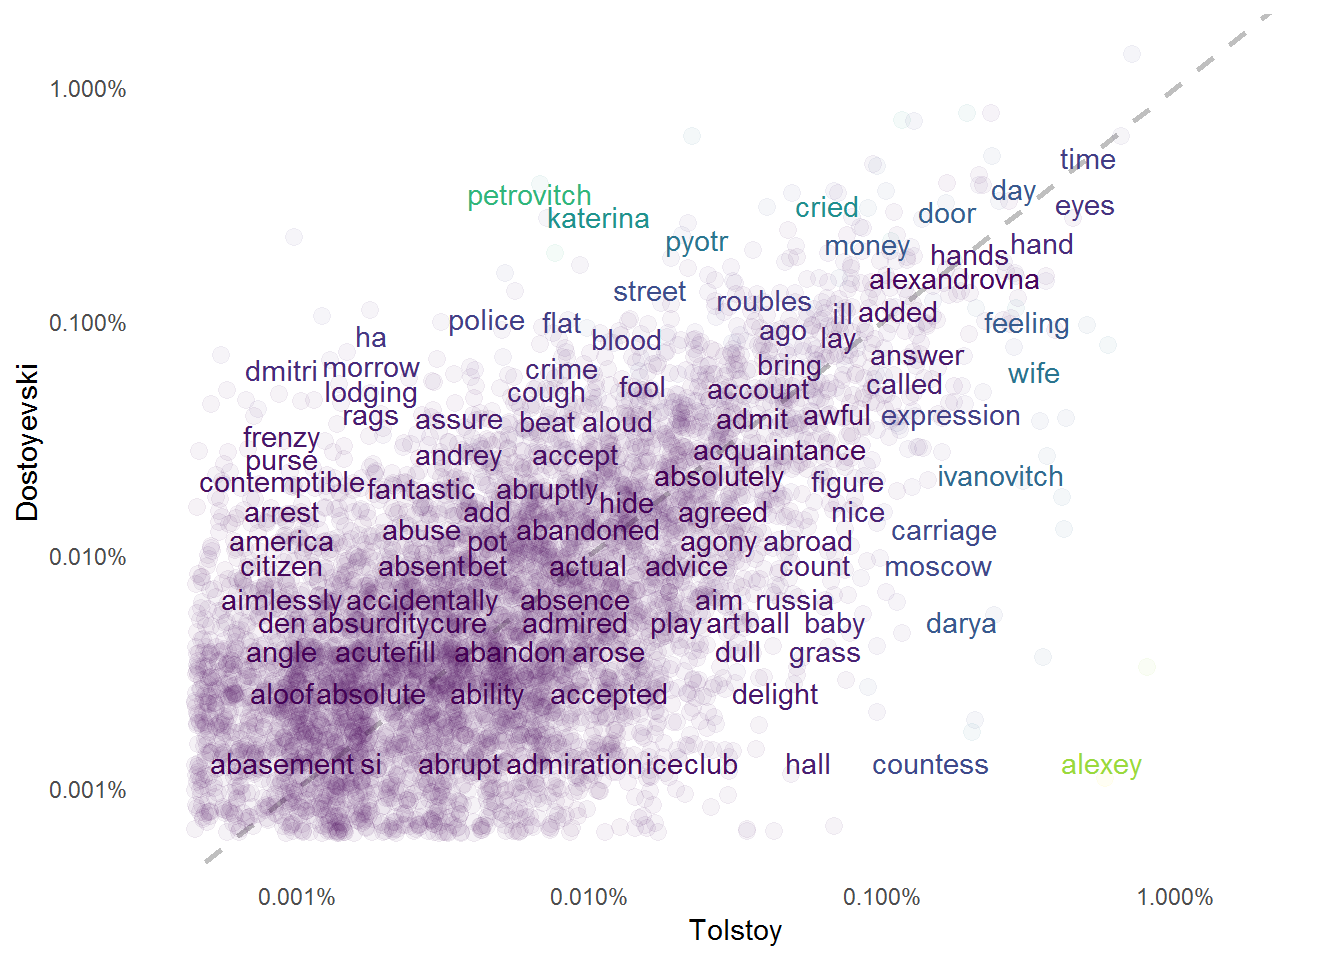
\includegraphics{2019-01-29-clustering-the-pharmaceutical-industry_files/figure-latex/unnamed-chunk-15-1.pdf}

\begin{Shaded}
\begin{Highlighting}[]
\CommentTok{# sillhouette method}
\KeywordTok{fviz_nbclust}\NormalTok{(pharmaceuticals_tbl, }\DataTypeTok{FUNcluster =}\NormalTok{ kmeans, }\DataTypeTok{method =} \StringTok{"silhouette"}\NormalTok{)}
\end{Highlighting}
\end{Shaded}

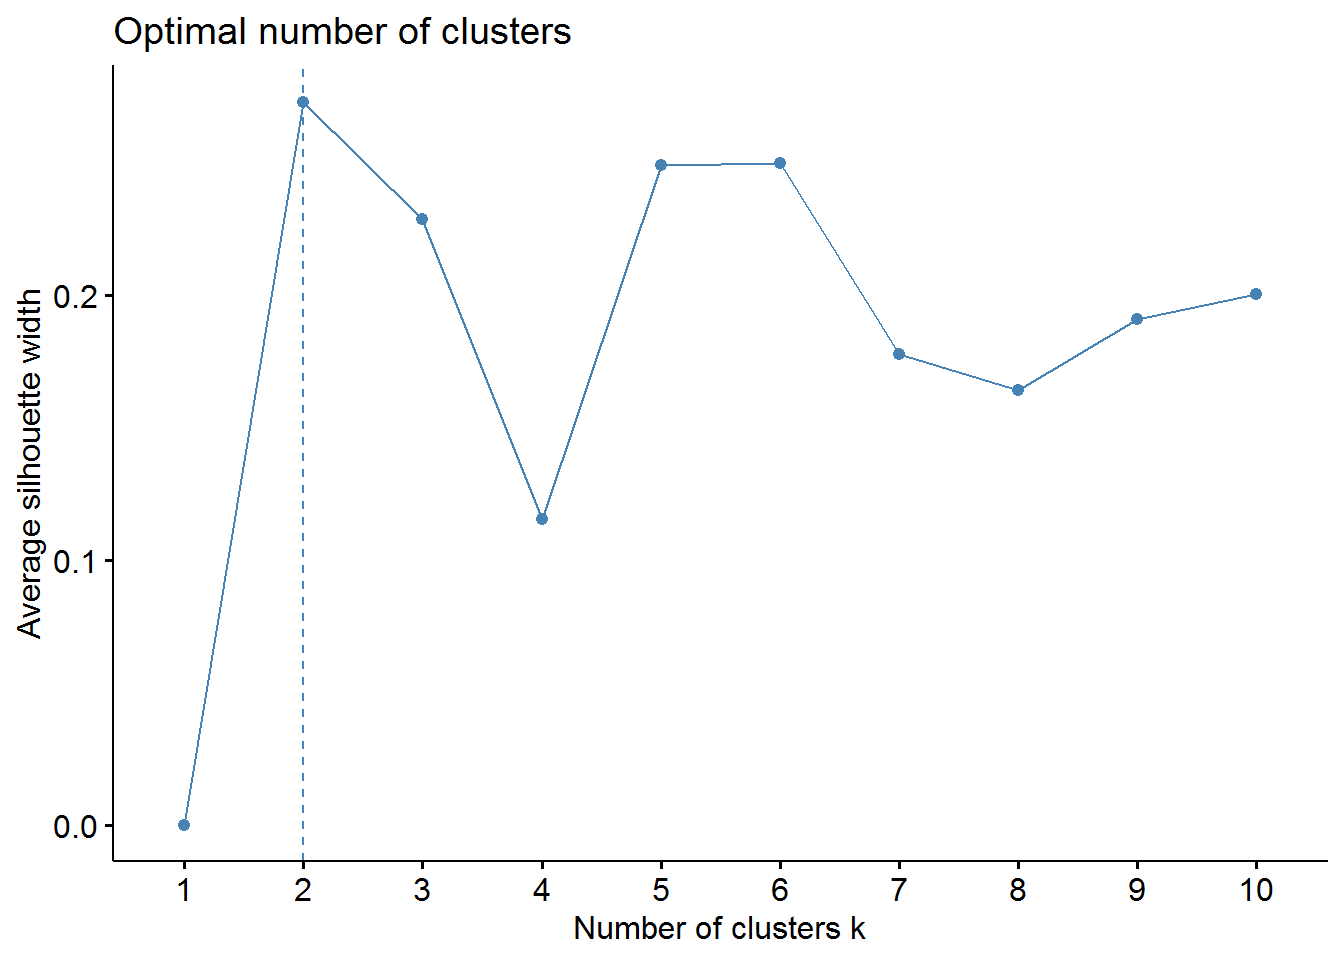
\includegraphics{2019-01-29-clustering-the-pharmaceutical-industry_files/figure-latex/unnamed-chunk-15-2.pdf}

From the elbow method we could choose 2, 3, or maybe 4 clusters.
However, the silhouette method indicates that 2 clusters correspond to
the optimal number.

Now, we can build our K-means cluster with two clusters.

\begin{Shaded}
\begin{Highlighting}[]
\KeywordTok{set.seed}\NormalTok{(}\DecValTok{88}\NormalTok{)}
\NormalTok{k_cluster2 <-}\StringTok{ }\KeywordTok{kmeans}\NormalTok{(pharmaceuticals_tbl, }\DataTypeTok{centers =} \DecValTok{2}\NormalTok{, }\DataTypeTok{nstart =} \DecValTok{50}\NormalTok{,}
                    \DataTypeTok{iter.max =} \DecValTok{10}\NormalTok{) }\CommentTok{# k equals 2 clusters}

\KeywordTok{table}\NormalTok{(k_cluster2}\OperatorTok{$}\NormalTok{cluster)}
\end{Highlighting}
\end{Shaded}

\begin{verbatim}
## 
##  1  2 
## 10 11
\end{verbatim}

As we have seen in the hierarchical clustering, we have 10
pharmaceutical in one cluster and 11 in the other one. Regardless, we
could check some metrics of compactness and separation with the function
\texttt{glance} from the \texttt{broom} package and with the
\texttt{dunn} function.

\begin{Shaded}
\begin{Highlighting}[]
\CommentTok{# check total within and between sum of squares}
\KeywordTok{glance}\NormalTok{(k_cluster2)}
\end{Highlighting}
\end{Shaded}

\begin{verbatim}
## # A tibble: 1 x 4
##   totss tot.withinss betweenss  iter
##   <dbl>        <dbl>     <dbl> <int>
## 1   180         119.      61.4     1
\end{verbatim}

\begin{Shaded}
\begin{Highlighting}[]
\CommentTok{# dunn index}
\NormalTok{dunn_k2 <-}\StringTok{ }\KeywordTok{dunn}\NormalTok{(}\DataTypeTok{clusters =}\NormalTok{ k_cluster2}\OperatorTok{$}\NormalTok{cluster, }\DataTypeTok{Data =}\NormalTok{ pharmaceuticals_tbl)}
\NormalTok{dunn_k2}
\end{Highlighting}
\end{Shaded}

\begin{verbatim}
## [1] 0.2546142
\end{verbatim}

We have a total within sum of squares (WSS) of 118.57 and between sum of
squares (BSS) of 66.67. The WSS is a measure of compactness where a
lower value is better, whereas BSS measures separation whose high value
reflects a better outcome. The dunn index is 0.30. A higher value is
considerably superior as the clusters are better separated and/ or more
compact.

We can now try to see if with 3 clusters our performance metrics will be
better. If so, we will segment our pharmaceutical with K equals 3.
First, we will build or K-means cluster.

\begin{Shaded}
\begin{Highlighting}[]
\KeywordTok{set.seed}\NormalTok{(}\DecValTok{88}\NormalTok{)}
\NormalTok{k_cluster3 <-}\StringTok{ }\KeywordTok{kmeans}\NormalTok{(pharmaceuticals_tbl, }\DataTypeTok{centers =} \DecValTok{3}\NormalTok{, }\DataTypeTok{nstart =} \DecValTok{50}\NormalTok{,}
                     \DataTypeTok{iter.max =} \DecValTok{10}\NormalTok{) }\CommentTok{# centers equals 3 clusters}



\KeywordTok{table}\NormalTok{(k_cluster3}\OperatorTok{$}\NormalTok{cluster)}
\end{Highlighting}
\end{Shaded}

\begin{verbatim}
## 
##  1  2  3 
##  6  4 11
\end{verbatim}

The table of this k-means clustering shows 6 pharmaceutical companies in
cluster 1, 4 in cluster 2, and 11 in cluster 3.

Now with the functions \texttt{glance} and \texttt{dunn} we will take a
look at the performance metrics.

\begin{Shaded}
\begin{Highlighting}[]
\CommentTok{# check wSS and BSS}
\KeywordTok{glance}\NormalTok{(k_cluster3)}
\end{Highlighting}
\end{Shaded}

\begin{verbatim}
## # A tibble: 1 x 4
##   totss tot.withinss betweenss  iter
##   <dbl>        <dbl>     <dbl> <int>
## 1   180         96.0      84.0     3
\end{verbatim}

\begin{Shaded}
\begin{Highlighting}[]
\KeywordTok{tidy}\NormalTok{(k_cluster3)}
\end{Highlighting}
\end{Shaded}

\begin{verbatim}
## # A tibble: 3 x 12
##       x1     x2     x3     x4     x5     x6     x7     x8     x9  size
##    <dbl>  <dbl>  <dbl>  <dbl>  <dbl>  <dbl>  <dbl>  <dbl>  <dbl> <int>
## 1 -0.826  0.478 -0.370 -0.563 -0.851 -0.999  0.850  0.916 -0.332     6
## 2 -0.613  0.270  1.31  -0.961 -1.02   0.231 -0.359 -0.576 -1.38      4
## 3  0.673 -0.359 -0.276  0.657  0.834  0.461 -0.333 -0.290  0.682    11
## # ... with 2 more variables: withinss <dbl>, cluster <fct>
\end{verbatim}

\begin{Shaded}
\begin{Highlighting}[]
\CommentTok{# check dunn index}
\NormalTok{dunn_k3 <-}\StringTok{ }\KeywordTok{dunn}\NormalTok{(}\DataTypeTok{clusters =}\NormalTok{ k_cluster3}\OperatorTok{$}\NormalTok{cluster, }\DataTypeTok{Data =}\NormalTok{ pharmaceuticals_tbl)}
\NormalTok{dunn_k3}
\end{Highlighting}
\end{Shaded}

\begin{verbatim}
## [1] 0.3076927
\end{verbatim}

The WSS shows a lower value and the BSS a higher value compared with the
K-means clustering with 2 clusters. The dunn index also has a higher
value which means that with K equals 3 the clusters are more separated
and have more compactness. In sum, the performance metrics of our
k-means algorithm seem to be better with 3 clusters than with 2.

Moving on in our analysis, now we will use a different approach from the
one described above where we used the \texttt{fviz\_cluster} function to
map our clusters in 2D format. In this case, we will use the UMAP
(Uniform Manifold Approximation and Projection) algorithm, which is a
dimension reduction algorithm similar to PCA. The UMAP algorithm reduces
the variables in a data frame with two columns/dimensions corresponding
to x and y coordinates. These two dimensions will capture the
variability of our data in a two-dimensional set. So, it becomes
possible to project in a two-dimensional graph the position of each
pharmaceutical companies in each cluster.

Firstly, we will use the use the function \texttt{umap} in our data
frame. The following step will be extracting the variable layout from
the UMAP object to create a data frame with the coordinates of the
respective pharmaceutical companies.

\begin{Shaded}
\begin{Highlighting}[]
\CommentTok{# umap our data frame}
\NormalTok{umap_pharma <-}\StringTok{ }\NormalTok{pharmaceuticals_tbl }\OperatorTok
\StringTok{  }\KeywordTok{umap}\NormalTok{()}

\CommentTok{# create umap dataframe}
\NormalTok{umap_obj <-}\StringTok{ }\NormalTok{umap_pharma}\OperatorTok{$}\NormalTok{layout }\OperatorTok
\StringTok{  }\KeywordTok{as.data.frame}\NormalTok{() }\OperatorTok
\StringTok{  }\KeywordTok{rownames_to_column}\NormalTok{(}\DataTypeTok{var =} \StringTok{"Pharma"}\NormalTok{)}

\NormalTok{umap_obj}
\end{Highlighting}
\end{Shaded}

\begin{verbatim}
##                                Pharma         V1          V2
## 1                 Abbott Laboratories -0.5599971  0.46196012
## 2                      Allergan, Inc.  0.9289384  1.43291560
## 3                        Amersham plc  0.3354541  0.34965708
## 4                     AstraZeneca PLC -0.5293549 -0.56448968
## 5                             Aventis  1.5377670 -0.09310394
## 6                            Bayer AG  0.9640006  0.72732919
## 7        Bristol-Myers Squibb Company -1.1071940 -0.01250234
## 8                        Chattem, Inc  0.5180765  1.05588066
## 9               Elan Corporation, plc  0.9458157 -0.47147116
## 10              Eli Lilly and Company -1.1430508  0.76003736
## 11                GlaxoSmithKline plc -1.4867707 -1.15857252
## 12                   IVAX Corporation  0.8873017  0.18199628
## 13                  Johnson & Johnson -1.1974953 -0.74347125
## 14 Medicis Pharmaceutical Corporation  1.2166261 -0.93939240
## 15                  Merck & Co., Inc. -0.7444749 -1.11176241
## 16                        Novartis AG -0.7579310  1.06683888
## 17                         Pfizer Inc -1.4173004 -1.53152437
## 18              Pharmacia Corporation  1.6203149  0.77533872
## 19        Schering-Plough Corporation -0.1964202  0.04833752
## 20       Watson Pharmaceuticals, Inc.  1.8203646 -0.47752432
## 21                              Wyeth -1.6346701  0.24352297
\end{verbatim}

We can also visualize the position of each pharmaceutical company in
this UMAP 2D projection.

\begin{Shaded}
\begin{Highlighting}[]
\CommentTok{# visualize umap dataframe}
\NormalTok{umap_obj }\OperatorTok
\StringTok{  }\KeywordTok{ggplot}\NormalTok{(}\KeywordTok{aes}\NormalTok{(V1, V2)) }\OperatorTok{+}
\StringTok{  }\KeywordTok{geom_point}\NormalTok{() }\OperatorTok{+}
\StringTok{  }\KeywordTok{geom_label_repel}\NormalTok{(}\KeywordTok{aes}\NormalTok{(}\DataTypeTok{label =}\NormalTok{ Pharma))}
\end{Highlighting}
\end{Shaded}

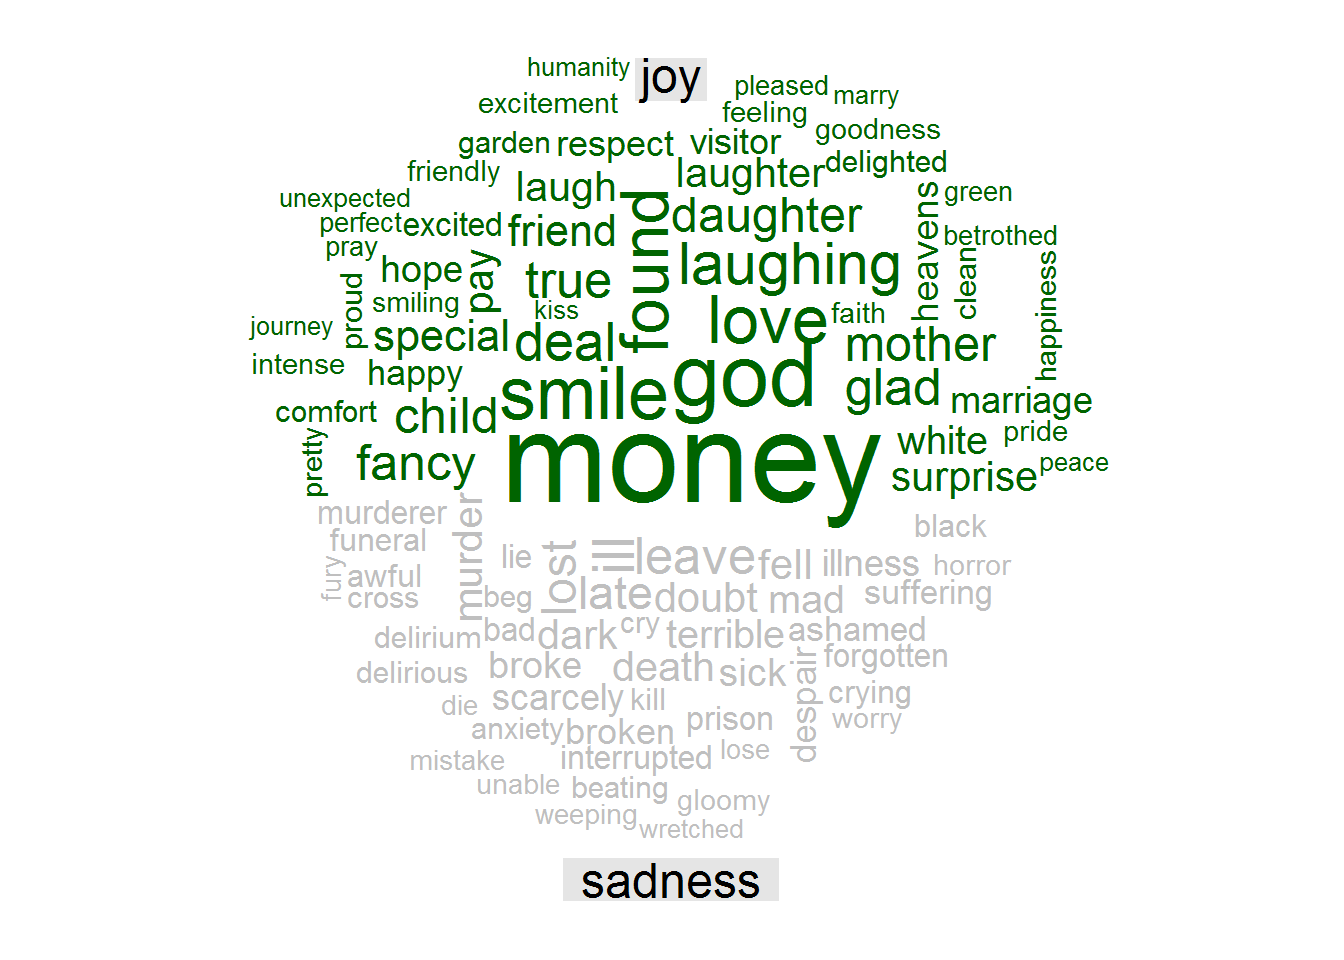
\includegraphics{2019-01-29-clustering-the-pharmaceutical-industry_files/figure-latex/unnamed-chunk-21-1.pdf}

Yet our goal is to map these pharmaceutical companies with the
respective cluster assignment. We will use \texttt{augment} from the
\texttt{broom} package to assign each cluster to our respective
pharmaceutical company. Right after , we will join the K-means data
frame with the \texttt{umap} object.

\begin{Shaded}
\begin{Highlighting}[]
\CommentTok{# use augment to assign the clusters to our pharmaceutical companies}
\NormalTok{kmeans_tbl <-}\StringTok{ }\KeywordTok{augment}\NormalTok{(k_cluster3, pharmaceuticals_tbl) }\OperatorTok\StringTok{ }
\StringTok{  }\NormalTok{dplyr}\OperatorTok{::}\KeywordTok{select}\NormalTok{(}\DataTypeTok{pharma =}\NormalTok{ .rownames, .cluster)}

\CommentTok{# join the kmeans data frame with the umap object}
\NormalTok{kmeans_umap <-}\StringTok{ }\NormalTok{kmeans_tbl }\OperatorTok\StringTok{ }
\StringTok{  }\KeywordTok{left_join}\NormalTok{(umap_obj, }\DataTypeTok{by =} \KeywordTok{c}\NormalTok{(}\StringTok{"pharma"}\NormalTok{ =}\StringTok{ "Pharma"}\NormalTok{))}

\NormalTok{kmeans_umap}
\end{Highlighting}
\end{Shaded}

\begin{verbatim}
## # A tibble: 21 x 4
##    pharma                       .cluster     V1      V2
##    <chr>                        <fct>     <dbl>   <dbl>
##  1 Abbott Laboratories          3        -0.560  0.462 
##  2 Allergan, Inc.               2         0.929  1.43  
##  3 Amersham plc                 2         0.335  0.350 
##  4 AstraZeneca PLC              3        -0.529 -0.564 
##  5 Aventis                      1         1.54  -0.0931
##  6 Bayer AG                     2         0.964  0.727 
##  7 Bristol-Myers Squibb Company 3        -1.11  -0.0125
##  8 Chattem, Inc                 1         0.518  1.06  
##  9 Elan Corporation, plc        1         0.946 -0.471 
## 10 Eli Lilly and Company        3        -1.14   0.760 
## # ... with 11 more rows
\end{verbatim}

Now, we can visualize the clusters in a 2D projection.

\begin{Shaded}
\begin{Highlighting}[]
\NormalTok{kmeans_umap }\OperatorTok\StringTok{ }
\StringTok{  }\KeywordTok{mutate}\NormalTok{(}\DataTypeTok{label_pharma =} \KeywordTok{str_glue}\NormalTok{(}\StringTok{"Company: \{pharma\}}
\StringTok{                                 Cluster:\{.cluster\}"}\NormalTok{)) }\OperatorTok
\StringTok{  }\KeywordTok{ggplot}\NormalTok{(}\KeywordTok{aes}\NormalTok{(V1, V2, }\DataTypeTok{color =}\NormalTok{ .cluster)) }\OperatorTok{+}
\StringTok{  }\KeywordTok{geom_point}\NormalTok{() }\OperatorTok{+}
\StringTok{  }\KeywordTok{geom_label_repel}\NormalTok{(}\KeywordTok{aes}\NormalTok{(}\DataTypeTok{label =}\NormalTok{ label_pharma), }\DataTypeTok{size =} \FloatTok{2.5}\NormalTok{) }\OperatorTok{+}
\StringTok{  }\KeywordTok{guides}\NormalTok{(}\DataTypeTok{color =} \OtherTok{FALSE}\NormalTok{) }\OperatorTok{+}
\StringTok{  }\KeywordTok{theme_minimal}\NormalTok{() }\OperatorTok{+}
\StringTok{  }\KeywordTok{scale_color_tq}\NormalTok{() }\OperatorTok{+}
\StringTok{  }\KeywordTok{labs}\NormalTok{(}\DataTypeTok{title =} \StringTok{"Pharmaceutical Companies Segmentation"}\NormalTok{,}
       \DataTypeTok{subtitle =} \StringTok{"K-Means Cluster Algorithm with UMAP Projection"}\NormalTok{)}
\end{Highlighting}
\end{Shaded}

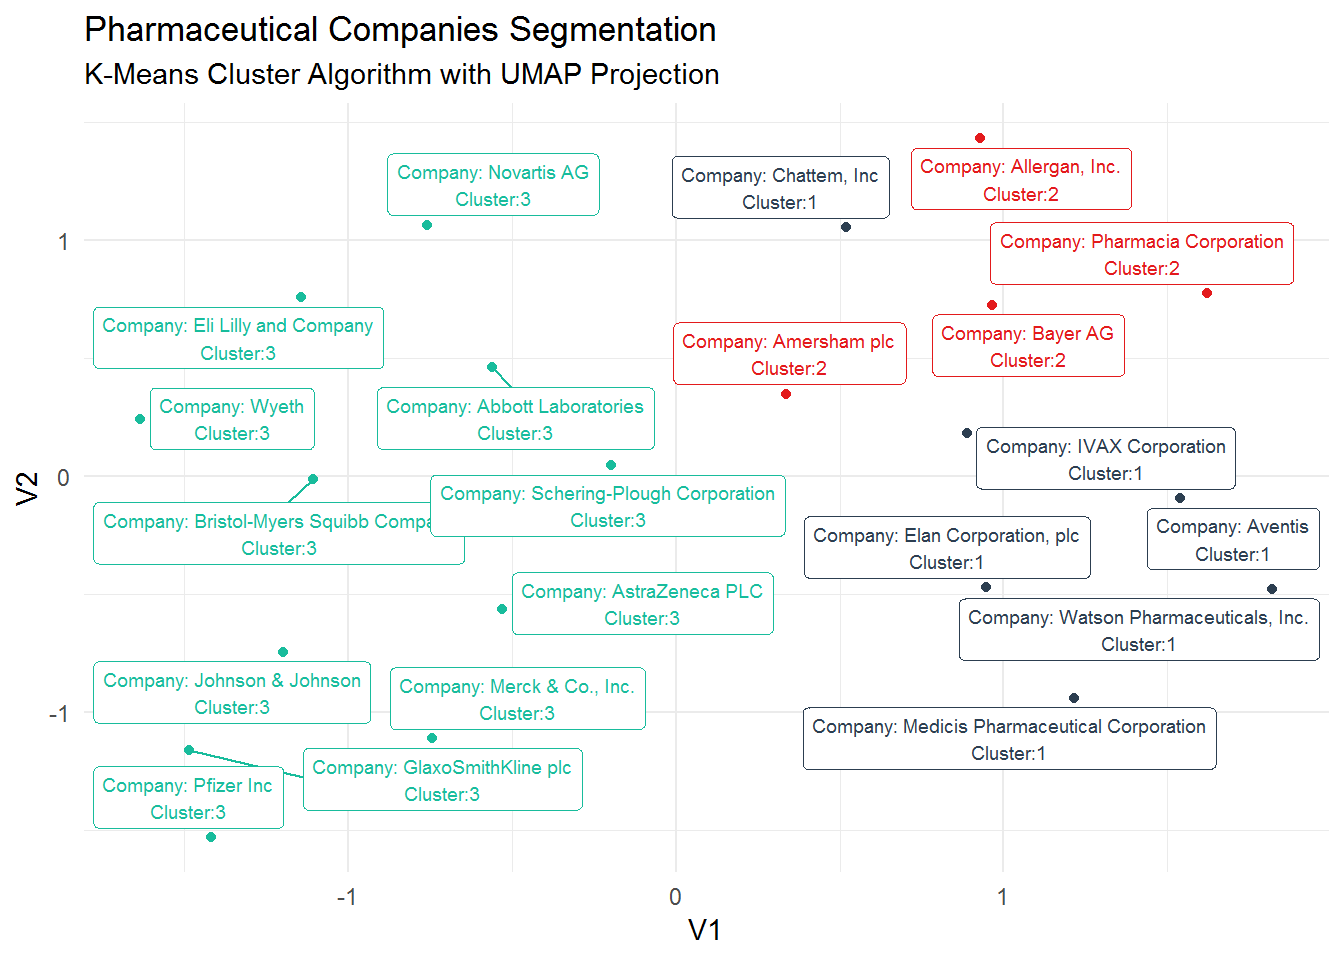
\includegraphics{2019-01-29-clustering-the-pharmaceutical-industry_files/figure-latex/unnamed-chunk-23-1.pdf}

As we did in the hierarchical clustering analysis, we need to check
which are the characteristics associated with each cluster. So, we still
need to find the real meaning of these clusters. We will use again the
\texttt{augment} function to create a data frame of our K-means
algorithm and find out how the variables profile in each cluster.

\begin{Shaded}
\begin{Highlighting}[]
\NormalTok{k_cluster3 }\OperatorTok
\StringTok{  }\KeywordTok{augment}\NormalTok{(pharmaceuticals_tbl) }\OperatorTok
\StringTok{  }\NormalTok{dplyr}\OperatorTok{::}\KeywordTok{select}\NormalTok{(}\OperatorTok{-}\NormalTok{.rownames) }\OperatorTok
\StringTok{  }\KeywordTok{group_by}\NormalTok{(.cluster) }\OperatorTok\StringTok{ }
\StringTok{  }\KeywordTok{summarise_all}\NormalTok{(mean)}
\end{Highlighting}
\end{Shaded}

\begin{verbatim}
## # A tibble: 3 x 10
##   .cluster Market_Cap   Beta PE_Ratio    ROE    ROA Asset_Turnover Leverage
##   <fct>         <dbl>  <dbl>    <dbl>  <dbl>  <dbl>          <dbl>    <dbl>
## 1 1            -0.826  0.478   -0.370 -0.563 -0.851         -0.999    0.850
## 2 2            -0.613  0.270    1.31  -0.961 -1.02           0.231   -0.359
## 3 3             0.673 -0.359   -0.276  0.657  0.834          0.461   -0.333
## # ... with 2 more variables: Rev_Growth <dbl>, Net_Profit_Margin <dbl>
\end{verbatim}

Cluster 3 shows a similar pattern as Cluster 1 from the Hierarchical
Clustering algorithm. It is comprised of high profitable companies
representing a low risk investment. Cluster 2 is composed of non-profit
companies and overpriced stocks showing a high volatility (high
Beta).Additionally, these companies do not seem to borrow a lot of money
(low Leverage). Cluster 1 includes non-profit and high volatility
companies as the companies in Cluster 2, and even considering revenue
growth and high levels of borrowings, their stocks look underpriced.

Let's create a tibble with the \texttt{tribble} function with the
cluster number and the respective characteristics.

\begin{Shaded}
\begin{Highlighting}[]
\CommentTok{# create tibble withthe characteristics of the 3 cluster}
\NormalTok{cluster_tibble <-}\StringTok{ }\NormalTok{tibble}\OperatorTok{::}\KeywordTok{tribble}\NormalTok{(}\OperatorTok{~}\NormalTok{.cluster, }\OperatorTok{~}\NormalTok{cluster.label,}
                                  \DecValTok{1}\NormalTok{, }\StringTok{"Non Profitable/High Risk Investment/Underpriced Stocks"}\NormalTok{,}
                                  \DecValTok{2}\NormalTok{, }\StringTok{"Non Profitable/High Risk Investment/Overpriced Stocks"}\NormalTok{,}
                                  \DecValTok{3}\NormalTok{, }\StringTok{"Profitable/Low Risk Investment"}\NormalTok{)}


\CommentTok{# make .cluster variable a factor}
\NormalTok{cluster_tibble <-}\StringTok{ }\NormalTok{cluster_tibble }\OperatorTok
\StringTok{  }\KeywordTok{mutate}\NormalTok{(}\DataTypeTok{.cluster =} \KeywordTok{as.factor}\NormalTok{(}\KeywordTok{as.character}\NormalTok{(.cluster)))}
\end{Highlighting}
\end{Shaded}

Now, we can visualize the clusters with respective description of such
characteristics.

\begin{Shaded}
\begin{Highlighting}[]
\CommentTok{# clusters visualization}
\NormalTok{kmeans_umap }\OperatorTok
\StringTok{  }\KeywordTok{left_join}\NormalTok{(cluster_tibble) }\OperatorTok
\StringTok{  }\KeywordTok{mutate}\NormalTok{(}\DataTypeTok{label_pharma =} \KeywordTok{str_glue}\NormalTok{(}\StringTok{"Company: \{pharma\}}
\StringTok{                                 Cluster:\{.cluster\}}
\StringTok{                                 \{cluster.label\}"}\NormalTok{)) }\OperatorTok
\StringTok{  }\KeywordTok{ggplot}\NormalTok{(}\KeywordTok{aes}\NormalTok{(V1, V2, }\DataTypeTok{color =}\NormalTok{ .cluster)) }\OperatorTok{+}
\StringTok{  }\KeywordTok{geom_point}\NormalTok{() }\OperatorTok{+}
\StringTok{  }\KeywordTok{geom_label_repel}\NormalTok{(}\KeywordTok{aes}\NormalTok{(}\DataTypeTok{label =}\NormalTok{ label_pharma), }\DataTypeTok{size =} \DecValTok{2}\NormalTok{) }\OperatorTok{+}
\StringTok{  }\KeywordTok{guides}\NormalTok{(}\DataTypeTok{color =} \OtherTok{FALSE}\NormalTok{) }\OperatorTok{+}
\StringTok{  }\KeywordTok{theme_tq}\NormalTok{() }\OperatorTok{+}
\StringTok{  }\KeywordTok{scale_color_tq}\NormalTok{() }\OperatorTok{+}
\StringTok{  }\KeywordTok{labs}\NormalTok{(}\DataTypeTok{title =} \StringTok{"Pharmaceutical Companies Segmentation"}\NormalTok{,}
       \DataTypeTok{subtitle =} \StringTok{"UMAP 2D Projection with the K-Means Cluster Algorithm"}\NormalTok{)}
\end{Highlighting}
\end{Shaded}

\begin{verbatim}
## Joining, by = ".cluster"
\end{verbatim}

\begin{verbatim}
## Warning: Column `.cluster` has different attributes on LHS and RHS of join
\end{verbatim}

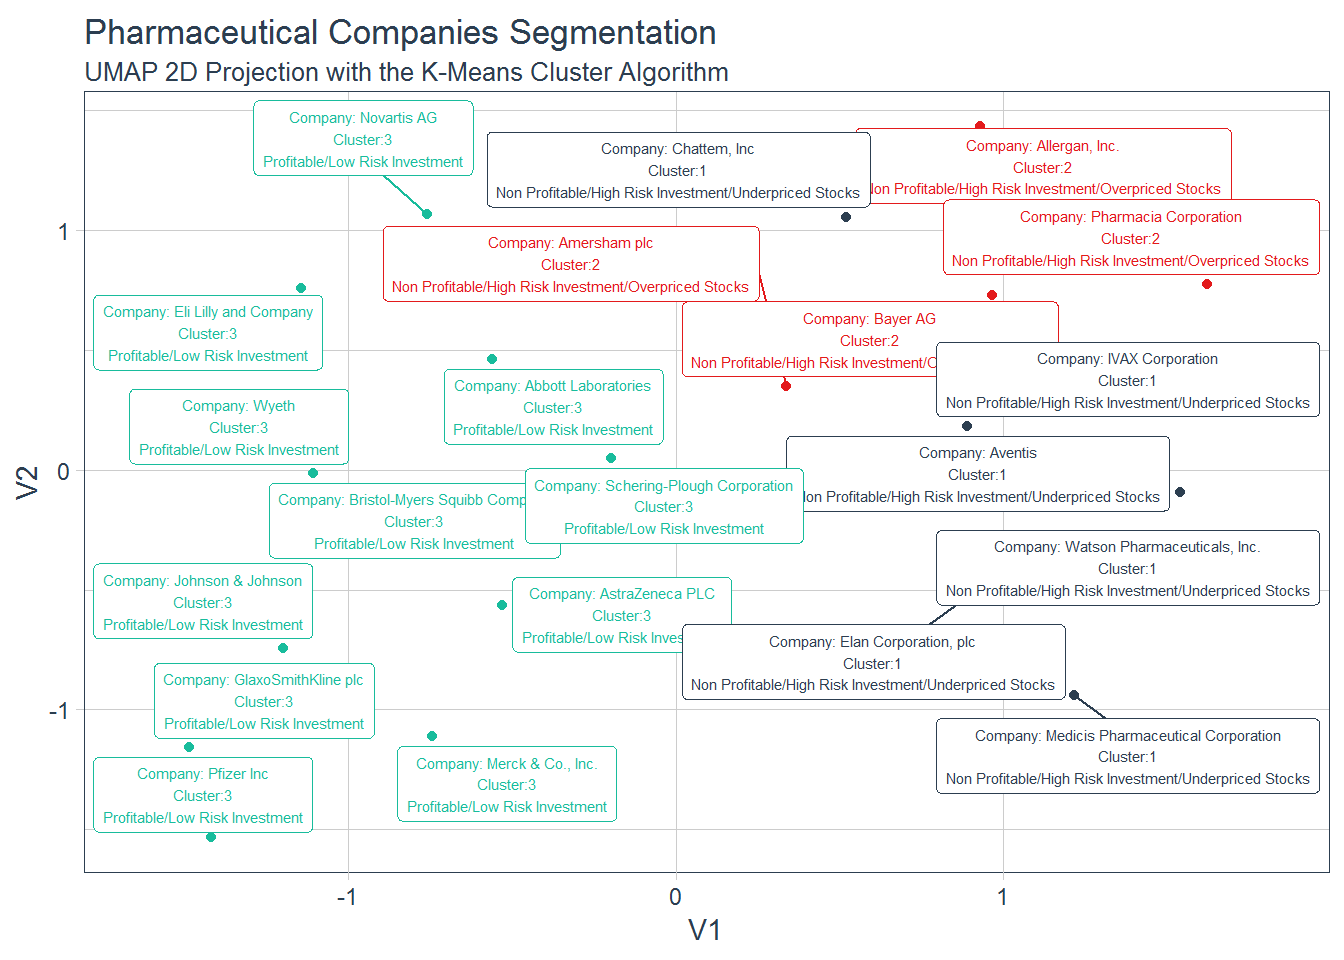
\includegraphics{2019-01-29-clustering-the-pharmaceutical-industry_files/figure-latex/unnamed-chunk-26-1.pdf}

\subsection{Conclusion}\label{conclusion}

Hope you have enjoyed this introduction to clustering analysis. Despite
the plethora of cluster algorithms, the goal was to show the power of
this unsupervised algorithm to segment any kind of business. Talk to you
through the following posts. in the meantimekeep coding!


\end{document}
